\documentclass[lettersize,journal]{IEEEtran}
\usepackage{amsmath,amsfonts}
\usepackage{algorithmic}
\usepackage{algorithm}
\usepackage{array}
\usepackage[caption=false,font=normalsize,labelfont=sf,textfont=sf]{subfig}
\usepackage{textcomp}
\usepackage{stfloats}
\usepackage{url}
\usepackage{verbatim}
\usepackage{amssymb}
\usepackage{graphicx}
\usepackage{tabularx}
\usepackage{cite}
\usepackage{bbm}
\usepackage{pifont}
\usepackage{booktabs}
\usepackage{makecell}
\usepackage[normalem]{ulem}
\newcommand{\cmark}{\ding{51}}%
\newcommand{\xmark}{\ding{55}}%
\usepackage{xcolor}
\newcommand{\red}[1]{\textcolor{red}{#1}}
\newcommand{\ul}[1]{\underline{#1}}
\newcommand{\Id}{\mathbbm{1}}

\newcommand{\st}[1]{\sout{#1}}
% NOTE: \us was used throughout the source but never defined; defined here.
\newcommand{\us}{\ensuremath{\mu}s}
\hyphenation{op-tical net-works semi-conduc-tor IEEE-Xplore}

% ---------------------------------------------------------------------------
% Float placement parameters. This paper carries an unusually high ratio of
% floats to text in Sections V-VII; the LaTeX defaults (topfraction 0.7,
% topnumber 2, totalnumber 3) cause oversized [t]-only floats to be deferred
% indefinitely and flushed at \end{document}, i.e. after the bibliography.
\renewcommand{\topfraction}{0.9}
\renewcommand{\bottomfraction}{0.7}
\renewcommand{\textfraction}{0.07}
\renewcommand{\floatpagefraction}{0.7}
\setcounter{topnumber}{3}
\setcounter{bottomnumber}{2}
\setcounter{totalnumber}{5}
% ---------------------------------------------------------------------------

\begin{document}

\title{From Sensing to Anticipation: Generative   \\
Waveform Models for Sub-Frame Dynamic \\
Spectrum Sharing}

\author{Chaoyi~He,
        Arya~Menon,
        Jacdon~Green,
        Linda~P.~B.~Katehi,~\IEEEmembership{Life~Fellow,~IEEE}%

\thanks{The authors are with the Department of Electrical and Computer
Engineering, Texas A\&M University, College Station, TX 77843 USA
(e-mail: katehi@tamu.edu).}
\thanks{This work was funded by a Texas A\&M CRI Grant.}}

% The paper headers
\markboth{Proceedings of the IEEE}{He \MakeLowercase{\textit{et al.}}: Generative Waveform Models for Sub-Frame Dynamic Spectrum Sharing}

\maketitle

%===================================================================== ABSTRACT
\begin{abstract}
Radio spectrum today is sensed, allocated, and reallocated in timescales of
seconds, minutes to hours, while the traffic that actually occupies it changes on
timescales of microseconds. This mismatch spans five or more orders of
magnitude and contributes to spectrum under-utilization as repeatedly
documented by measurements; a band recorded as ``busy'' is
typically busy only partly and intermittently. This paper argues
that improving spectrum utilization requires moving from \emph{sensing}
the spectrum in its past or present utilization to \emph{anticipating} what it
will do in useful future time segments at the resolution of individual
physical-layer frames, and that generative sequence models operating on raw
complex baseband waveforms are a credible means to achieving these goals.

We present this argument in three parts. First, we provide a tutorial
survey of modeling and prediction methods of spectrum occupancy, starting
with measurement-driven Markov and semi-Markov models, through
autoregressive time-series methods, classical machine learning and deep
sequence models, to transformer-based long-horizon predictors. We
organize this literature by three structural choices that determine
what a predictor can and cannot do: the observable spectrum, the
temporal resolution at which it observes, and whether it represents user
arrival and departure as a stochastic process. Second, we give a
short and self-contained tutorial of the two machine learning
components that a waveform-level predictor requires---contrastive
self-supervised representation learning and denoising diffusion
probabilistic models. The tutorial is written for a wireless engineer
rather than a machine learning specialist, and, as such, we focus on
orthogonal frequency-division multiplexing (OFDM) waveforms for which we
identify the properties and the shape of the tools we must adapt to enhance the
sensing algorithms capable of prediction. Third, we present a complete
reference architecture and evaluate it, as a case study, on an IEEE 802.11ax
set of 30 simulated indoor channel realizations and on over-the-air
recordings from software-defined radios. The architecture predicts the
occupancy of eight 10~MHz sub-blocks within an 80~MHz band at the
granularity of the 12.8-$\mu$s useful portion of an OFDM symbol, excluding the guard interval. 
This prediction interval is four or more orders of magnitude shorter than 
the intervals used by most methods surveyed.

This case study yields an outcome, which we consider more instructive than a
headline score.
In the evaluation windows where occupancy actually changes, the generative stage
\emph{on its own} does not outperform a predictor driven by a conventional
sensing algorithm (AUC 0.819 versus 0.850).
However, when fused with the sensed estimate, it achieves an AUC of 0.884 and an
average precision of 0.947, compared with a limit of 0.897 for the same
classifier given the true future waveform.
Sensing and predicting are therefore complementary rather than competing: the
sampled futures carry information about impending transitions that the
current state does not contain, and this information is only realized in the
future.
We incorporate this information and four further findings into design
principles, and we create an evaluation protocol which includes
transition-conditioned windows, sensed-persistence baselines, and
collision-referenced operating points---that we argue the field should adopt,
because aggregate metrics computed over randomly drawn windows are dominated by
the trivially predictable and may conceal the absence of any predictive
skill at all.
What stands between this class of predictive method and algorithmic deployment
is an inference latency that is currently three orders of magnitude too large
compared to the predictive window, unmodeled hardware imperfections and
impairments, the absence of shared benchmarks, adversarial vulnerability, and
the standards and regulatory interfaces through which any sub-frame sharing
scheme must eventually operate.
\end{abstract}

%========================================================================================================= INTRODUCTION
\section{\textbf{INTRODUCTION}}
\IEEEPARstart{W}{ireless} spectrum is the substrate on which a growing
fraction of economic and social activities run.
Cellular networks, wireless local area networks, satellite constellations, UAVs,
radars, and an expanding population of embedded and Internet-of-Things devices
all draw on the same finite and extremely limited spectrum resource, while at
the same time demand has grown faster than the supply of newly cleared bands
\cite{Azmat2015, Rahman2021, Piran2020, Chen2022}.
The consequences are familiar to every user: contention, latency,
retransmission, and failed or abruptly terminated connections in dense
environments.

The engineering response of the past two decades has been to make
allocation more dynamic. Cognitive radio proposed that devices sense
their environment and adapt \cite{Mitola1999, Haykin2005}; regulators
built frameworks, of which the three-tier Citizens Broadband Radio
Service is the most fully realized, where a database or spectrum
access systems grant and revoke rights on demand \cite{FCC2015CBRS};
and national spectrum policies have increasingly considered sharing rather
than clearing as the primary route to additional capacity
\cite{NSS2023}.
These are real advances, which also share a common temporal characteristic:
they operate within the spectrum bands granted by an access system, where these
bands are indicated as unavailable for seconds, minutes, or longer (see Fig.~\ref{fig_0}).

%%----------------------------------------------------------------------------------SUBSECTION INTRO-A
\subsection{\textbf{The Granularity Gap}}
The traffic that actually occupies a band does not always correlate with the
previously mentioned timescale.
In an IEEE802.11ax network, the atomic unit of transmission
is an OFDM symbol which lasts about 13~$\mu$s, and the multi-user
extension of OFDM, OFDMA, subdivides the band into resource units that
are assigned and released packet by packet. A station that has been granted an
80~MHz channel, at any given time, may be using two of its eight 10~MHz
sub-blocks with the remaining six physically available.
However, they become unavailable only because the allocation access system does
not include them.

%======================================================================= FIG. 1
\begin{figure*}[!t]
\centering
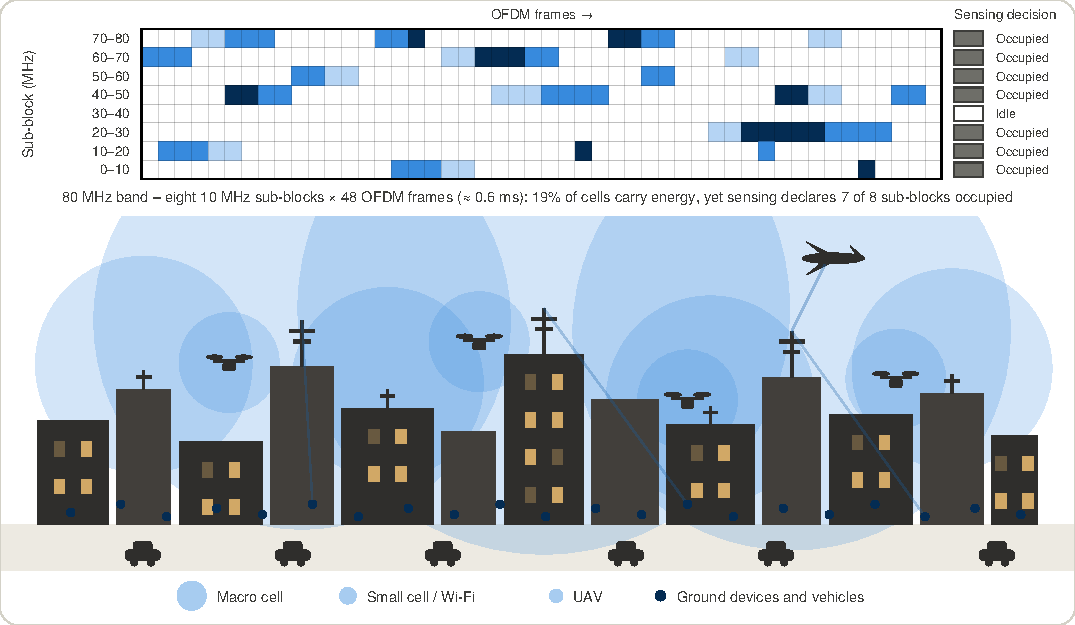
\includegraphics[width=\textwidth]{Fig/fig0_congested_urban_spectrum.pdf}
\caption{The gap this paper addresses. Above: an 80~MHz band - eight 10 MHz 
sub-blocks x 48 OFDM-symbol intervals (614.4 $\mu$s, excluding guard intervals),
shaded by received power; the column at right gives the occupancy a single sensing
decision reports over the same window. Below: the environment that produces
this pattern, in which overlapping macro-cell, small-cell, aerial and ground
transmissions contend for the same band. Sensing resolves seven of the eight
sub-blocks as occupied; at OFDM-symbol resolution, fewer than one fifth of the
time--frequency cells carry energy.}
\label{fig_0}
\end{figure*}
%------------------------------------------------------

Fig.~\ref{fig_real} contrasts the two regimes.
In the conventional arrangement, the spectrum held by an
ongoing transmission is reallocated only once that
transmission has completed, so the interval between a user's
last symbol and the next user's first is unutilized time and is repeated at
every handover.
In the anticipatory arrangement, the end of one transmission
and the onset of the next are predicted before they occur, and the
reallocation is prepared in advance. The distinction is not a matter of
efficiency at the margin: it determines whether a heterogeneous
device---a radar return pulse, a satellite up-link or a sensor report---can occupy
a vacant sub-block at all, or must wait for the entire band to be
released.

%======================================================================= FIG. 2
\begin{figure*}[!t]
\centering
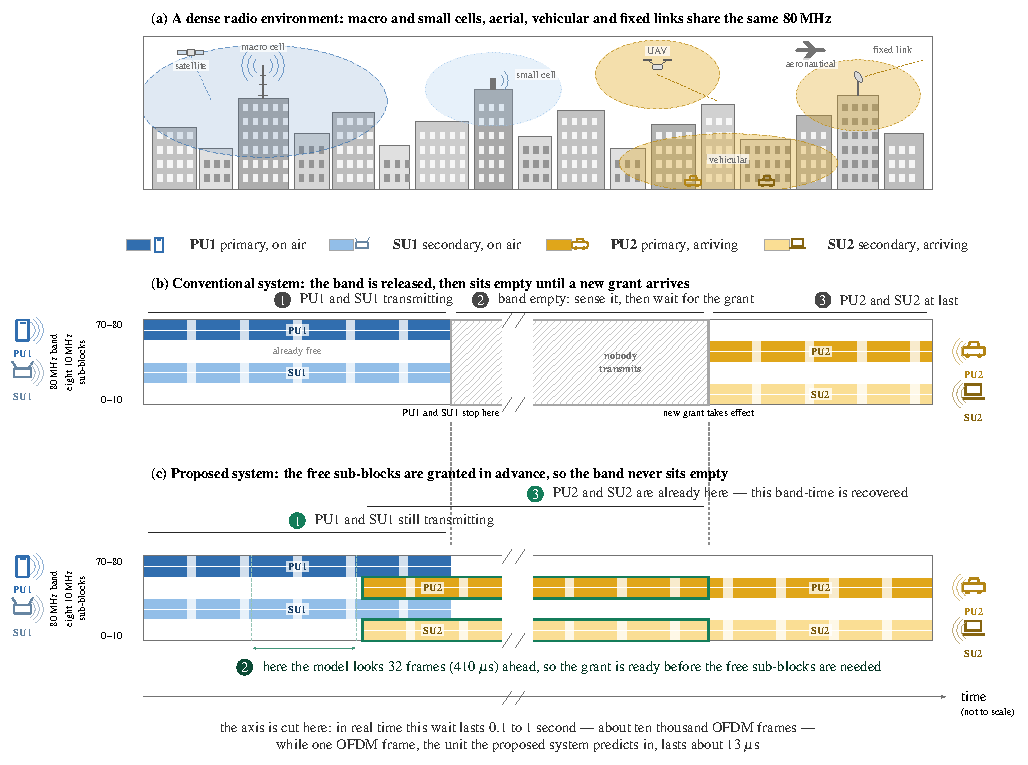
\includegraphics[width=6.5in]{Fig/fig_real.pdf}%
\caption{Comparison between the conventional spectrum allocation system and the
proposed system utilizing a diffusion model for time-domain signal prediction. 
The top section shows various devices (including primary
users PU1 and PU2 and secondary users SU1 and SU2) communicating via cell tower and satellite links.}
The middle section illustrates the conventional system, where spectrum allocation waits
for ongoing communications (e.g., PU1, SU1) to conclude before reallocating spectrum,
resulting in inefficiencies. In contrast, the section shows the proposed system,
in which the diffusion model predicts the end of current communications and the start
of new ones (PU2, SU2), enabling dynamic reallocation of spectrum resources.
This proactive reallocation enhances spectrum utilization by reducing waiting times
and optimizing the allocation phase.
\label{fig_real}
\end{figure*}
%==============================================================================

We refer to this as the \emph{Granularity Gap}: the difference between
the resolution at which spectrum is managed and the resolution at which
it is used.
Measurement campaigns have consistently documented the consequences of this gap
for two decades, reporting that large portions of the
spectrum are used lightly, if not at all, even in bands nominally under
pressure, with a strong dependence on band, direction, location, and time of day
\cite{Chen2016, Wellens2007, Engiz2021, Kozlowski2021, Raouf2023}.
A common interpretation of these measurements is that there is
headroom.
Contrary to that, the interpretation we have adopted here is stronger:
\emph{"much of the headroom is invisible not because it is small
but because it is short-lived and narrow, and no operational system resolves it"}.
Throughout this paper, one prediction step corresponds to the 1024-sample useful 
portion of an IEEE802.11ax 
OFDM symbol sampled at 80 MS/s, giving a duration of 12.8 $\mu$s. 
The guard interval is removed before the model input is formed. 
We therefore use "OFDM symbol" for this unit and reserve 
"frame" and "packet" for PHY- or MAC-level structures 
containing one or more OFDM symbols. The 32-step prediction 
horizon is consequently 409.6$\mu$s

%----------------------------------------------------------------------------------SUBSECTION INTRO-B
\subsection{\textbf{Sensing, Prediction, Anticipation}}
Three capabilities must be distinguished, which are not 
always recognized and distinguished by the literature. 

\emph{Sensing} presents what the spectrum is doing now.
Energy detection, matched filtering, cyclostationary feature detection,
and wavelet methods all address this problem, and, actually, they address it well
\cite{Yucek2009, Muzaffar2024, FontSegura2010, Tian2006}.
Sensing is, however, structurally retrospective: by the time a detector has
integrated enough energy to declare a sub-block vacant, the sub-block
may already have been reoccupied.

\emph{Prediction} speaks to what the spectrum will do over the next
interval, and has been the subject of a substantial literature reviewed in
Section~III.
Almost all of that literature predicts an
aggregate---a power level, a duty cycle, a binary occupancy
label---over an interval of hundreds of milliseconds to minutes.
That resolution supports strategic decisions, such as which band to camp on,
and it does so effectively.

\emph{Anticipation}, as we use the term, provides prediction at the resolution
of the events themselves, allowing for actions that can alter the outcome
within the time duration of the event, i.e., knowing that the transmission that
currently occupies sub-block 3 will end within the next several frames, and that
a new arrival will claim sub-block 5 shortly after.
This is the information a
secondary transmitter needs in order to occupy a gap without
colliding with the incumbent.
It requires a temporal resolution
comparable to the frame duration and a frequency resolution comparable
to the resource unit, and it requires an explicit model of the
stochastic process by which users arrive and depart.
%----------------------------------------------------------------------------------SUBSECTION INTRO-C
\subsection{\textbf{Why Generative, and Why Waveforms}}
Two commitments follow from the definition of anticipation, and we use them to
organize the technical content of this paper:

a) The required model should learn and recognize raw complex baseband
waveforms rather than learn from derived scalar summaries 
which mask information on a refined time scale.
A power measurement integrated over a channel and a millisecond has, by
construction, discarded the modulation structure, the preamble and padding
patterns, and the per-symbol resource-unit assignments from which the
imminent end of a transmission can be inferred.
These cues exist in the I/Q stream.
The cost of extracting and maintaining this refined information 
is severe: an 80~MHz band sampled at
Nyquist produces about $10^8$ complex samples per second, and
a five-second capture of the utilized spectral information yields a matrix of
$303\,459 \times 1024$ elements.
Any waveform-level predictor based on a data-reduction constraint,
makes representation learning not an optional refinement of the architecture
but a load-bearing component.

b) The model required to provide this refined information about the spectrum 
should be \emph{generative} rather than \emph{discriminative}.
User arrivals and departures are stochastic;
under the queueing model used later in this paper, they constitute a
time-varying Poisson process.
As a result, there is no single correct future
waveform that exists, and a regression trained to minimize squared error against the
realized future will converge toward the conditional mean, which for a
multimodal predictive distribution is a waveform that could and would not
physically occur.
Contrary to the above, a generative model draws samples from the
predictive distribution.
Each sample represents a physically plausible future and
their spread provides a calibrated statement about uncertainty. As a result,
downstream, the disagreement among samples about whether a sub-block
will be occupied is exactly the quantity a secondary user would need in
order to trade collision risk against throughput.
Denoising diffusion probabilistic models \cite{Ho2020, SohlDickstein2015, Song2021}
are well suited to this role because they are stable to train on
continuous-valued, high-dimensional signals and provide straightforward
conditioning on a learned context vector.
%----------------------------------------------------------------------------------SUBSECTION INTRO-D
\subsection{\textbf{Scope and Contributions}}
This paper is written for a reader who works in wireless systems and
wishes to understand whether, and under what conditions, generative
machine learning changes what is achievable in dynamic spectrum sharing.
It is not written for the machine learning specialist, and the tutorial
material in Sections~II, III and IV is presented accordingly. 
These sections include:

\textbf{\emph{A tutorial survey}} of spectrum prediction
(Section~III), organized not chronologically but by the three
structural choices---observable, resolution, and stochastic
modeling---that characterize what any given method can do. We use this
organization to locate where the granularity gap originates
in the existing literature.

\textbf{\emph{A tutorial treatment}} of the enabling machine learning
(Section~IV) that covers the concept of contrastive predictive coding 
and denoising
diffusion at a level sufficient for a wireless engineer to understand 
and assess available
design choices. In addition, this treatment provides an analysis 
of the properties of OFDM waveforms---
cyclic prefix structure, I/Q representation, symbol-level
symmetry---that require the above general-purpose tools to be adapted.

\textbf{\emph{A reference architecture}} (Section~V) that realizes
sub-frame anticipation as three interoperable stages, with each stage's
role, interface, and cost stated explicitly so each of these becomes an
alternative that can be substituted.

\textbf{\emph{An evaluation protocol}} (Section~VI) for
anticipatory spectrum prediction. We show that because occupancy dwell
times exceed plausible prediction horizons by three orders of magnitude,
metrics computed over randomly drawn evaluation windows are dominated by
windows containing no event, in which a trivial copy-forward predictor
is exact by construction. We propose the use of a transition-conditioned
evaluation combined with sensed-persistence baselines, and reporting at a
collision-referenced operating point, and we assess how much
apparent but rather incorrect performance these corrections remove.

\textbf{\emph{An empirical case study}} (Section~VII) on 30 simulated
802.11ax channel realizations and on over-the-air software-defined radio
recordings, reported under that protocol, including a zero-shot transfer
experiment to environments withheld from the generative stage.
The central empirical finding of
the case study is partly negative, indicating that the generative 
stage alone does not outperform a well-constructed conventional 
baseline. However, we report it prominently because we believe that 
the field is at a stage where an honest accounting of what generative 
models do and do not contribute is more valuable than another 
incremental score. At the same time the accompanying
positive finding---that generation and sensing are strongly
complementary---is only appreciated and interpretable alongside 
the above recognition.

\textbf{\emph{Design principles and a research agenda}}
(Sections~VIII and IX), that includes a latency budget to quantify
the gap between the present implementation and real-time operation, and
an assessment of the standards, regulatory, benchmarking, and security
work that sub-frame sharing would require.

\subsection{\textbf{Organization of the Following Sections}}
Section~II defines and characterizes spectrum occupancy as an object of
measurement and modeling, while establishing the timescale ladder on which
the rest of the paper is positioned. Section~III surveys spectrum
prediction. Section~IV develops the machine learning foundations.
Section~V presents the reference architecture and Section~VI the
evaluation methodology. Section~VII reports the case study.
Section~VIII abstracts design principles, Section~IX sets out
open problems, and Section~X concludes.

%============================================================================================================ SECTION II
\section{\textbf{Spectrum Occupancy as an Object of Measurement and Modeling}}

Before surveying prediction methods, we should define what
we mean by prediction and what is being predicted.
This is necessary because in the literature, implicit 
answers about prediction differ much more than the 
methods utilized to derive these predictions.
%----------------------------------------------------------------------------------SUBSECTION II-A
\subsection{\textbf{Dimensions of Occupancy}}
Occupancy is not represented by a scalar, but 
by a multidimensional vector.
A band may be occupied in time, in frequency,
in space, in code, and/or in angle of arrival, 
and a resource is genuinely
available to a secondary user only if it is free 
in each and every dimension that
the secondary user's own transmission would require \cite{Yucek2009}.
Most of the prediction literature, including this paper, treats the joint
time--frequency problem, with spatial reuse handled either implicitly
through the propagation model or explicitly by predictors that learn from
measurements derived from multiple locations \cite{Li2021, Ren2021, Shawel2019}.
Angle- and code-domain occupancy, which massive multiple-input
multiple-output and non-orthogonal access make increasingly relevant,
are largely absent from the prediction literature and represent a real
gap.
%----------------------------------------------------------------------------------SUBSECTION II-B
\subsection{\textbf{What Measurement Campaigns Established}}
Large-scale measurement data provide an empirical foundation for the
entire field \cite{Chen2016}.
Their cumulative findings can be summarized in three statements:
(a) Occupancy remains highly heterogeneous across bands and directions.
For example, as of recent urban measurements of U.S. LTE and 5G
bands, downlink channels exhibit substantially higher occupancy than
uplink, while the Citizens Broadband Radio Service and 5Gn77 bands stand
out as markedly less occupied than other studied cellular bands
\cite{Raouf2023}.
Occupancy is also highly heterogeneous across location and
time, so that a single number for a band is nearly meaningless
\cite{Wellens2007, Engiz2021, Kozlowski2021}.
As a result, the aggregate duty cycle, the most commonly reported statistic,
is acutely sensitive to detection threshold and receiver placement, which limits
its comparability with existing measurement sets \cite{Wellens2010}.

The last point deserves special emphasis because it recurs in the machine
learning literature in a different guise.
A predictor algorithm trained on labels produced by a thresholded energy
detector inherits that detector's threshold sensitivity; its reported accuracy
reflects a particular labeling convention rather than physical occupancy.
Waveform-level methods do not eliminate this problem, as labels
must still come from somewhere, but they at least allow the labeling
function to be a learned classifier applied to the full signal rather
than a scalar comparison.
%----------------------------------------------------------------------------------SUBSECTION II-C
\subsection{\textbf{The Timescale Ladder}}
Table~\ref{tab:timescales} arranges spectrum decisions by the timescale
on which they can be made.
The entries span roughly ten orders of
magnitude, from multi-year licensing to the OFDM symbol.
Two features of this ladder are worth noting.

First, the surveyed prediction literature clusters in the middle of the
ladder, at $10^{-1}$ to $10^{3}$~s.
This is not accidental: it is the
range over which power and duty-cycle observables are meaningful and
over which the aggregate statistics of a user population are stable.

Second, the events that create sub-block vacancies live at the bottom of
the ladder.
A transmission ends at a frame boundary.
In the data sets used in this paper, occupancy dwell times fall in
the 0.1--1~s range while the prediction horizon is 32 frames,
approximately 410~\us.
The ratio between the two is roughly $10^{3}$.
This ratio is consequential for evaluation, an issue discussed in
Section~VI: pointing to the observation that within a randomly selected
window, nothing happens.

%===================================================================== TABLE I
\begin{table}[!t]
\centering
\caption{\textbf{The Spectrum Decision Timescale Ladder}}
\label{tab:timescales}
\renewcommand{\arraystretch}{1.2}
\begin{tabular}{@{}lll@{}}
\toprule
\textbf{Timescale} & \textbf{Decision} & \textbf{Mechanism} \\
\midrule
Years            & Band allocation        & Regulatory proceeding \\
Hours--days      & Coordination           & Database, coexistence \\
Seconds--min     & Grant assignment       & SAS, scheduler, handover \\
$10^{-1}$--$1$~s & Occupancy dwell        & User session \\
1~ms             & Packet/TXOP            & MAC contention \\
10--16~$\mu$s    & OFDM symbol            & PHY \\
\bottomrule
\end{tabular}
\end{table}

%----------------------------------------------------------------------------------SUBSECTION II-D
\subsection{\textbf{Statistical Structure and Its Implications for Learning}}
\label{sec:nested}
One structural characteristic of the occupant signal is easily overlooked and
materially affects how results should be assessed, as explained below.
Today's standards constrain allocation to be contiguous and quantized 
\red{\st{\i.e.} i.e.}, in 802.11ax, the band is divided into 20~MHz increments, 
so the eight 10~MHz occupancy indicators of an 80~MHz 
channel are not eight independent binary variables.
They form a small set of nested states, and the prediction task is better
described as forecasting the transition times of that nested state than as eight
independent classification problems.

This leads to two consequential attributes: (a) reported per-sub-block accuracies are
inflated relative to what an independent-label reading would suggest, 
and (b) any metric must be interpreted
against the base rate of the evaluation set rather than against 0.5.
We report base rates explicitly throughout Section~VII for this reason.

%=========================================================================================================== SECTION III
\section{\textbf{Spectrum Prediction: A Tutorial Survey}}

This section surveys the methods that have been developed specifically for
spectrum prediction.
We organize the survey by the three structural attributes identified in Section~I:
(a) the learned observable, (b) the achieved resolution, and
(c) whether user dynamics are modeled stochastically.
The resulting taxonomy is summarized in Table~\ref{tab:taxonomy}.
More information on additional methods is provided by the existing review
literature \cite{Yucek2009, He2010, Xing2013, Chen2016, Ding2018, Wang2024}.

%----------------------------------------------------------------------------------SUBSECTION III-A
\subsection{\textbf{Occupancy Models: Markov and Semi-Markov Processes}}
The earliest prediction methods grew directly out of the collected measurement
datasets.
If occupancy is observed to alternate between busy and idle,
the natural model is a two-state continuous-time Markov or semi-Markov
chain, in which the band switches between occupied and unoccupied states
according to empirically fitted transition probabilities, with dwell
times drawn from fitted holding-time distributions
\cite{Gibson1994, Percival1997}.
Refinements conditioned on the previous
state along with their adjacent channel state yield eight transition
probabilities rather than four \cite{Saad2016, Pan2026}.
Whenever the underlying process is naturally identified, discrete-time chains are
more appropriate in characterizing the event.

From a prediction standpoint, a practical formulation is based on a hidden
Markov model: the true channel state is not observed, only a noisy
detector output is identified, and the parameters of an often non-stationary
underlying chain must be learned while the hidden occupancy states are
inferred \cite{Chen2011, Akbar2007}.
Conventional HMM formulations target one-step-ahead prediction;
extension to multiple steps requires recasting the problem,
i.e., as maximum-likelihood classification over state sequences
\cite{Saad2016}. The chain may also be estimated by Bayesian inference
\cite{Xing2013b}, at the cost of sensitivity to the choice of prior
distributions \cite{Pan2026}.

The strength of this family of prediction algorithms is that it models accurately
the stochastic process, the third of the three structural
choices, explicitly, and it is the only classical family that does so.
Its weakness is dimensional: the state space is over a single band's
binary occupancy, and extending it jointly across frequency and space is
combinatorially very complex.

%----------------------------------------------------------------------------------SUBSECTION III-B
\subsection{\textbf{Time-Series Models: AR, MA, ARMA, ARIMA}}
Linear time-series models provide the dimensional flexibility that
Markov models lack. Building on Yule's autoregressive formulation
\cite{Yule1927} and Slutsky's moving-average representation
\cite{Slutsky1937}, Box and Jenkins unified the two into the ARMA family
and generalized it to the autoregressive integrated moving-average
(ARIMA) class \cite{Box1978}, in which the current value of a possibly
difference-series is a linear function of its own past values and past
shocks. All four models appear in the spectrum literature; the
mathematical statements are collected in \cite{Ding2018}.

Model selection follows the standard Box--Jenkins diagnostic. By writing
the model as ARIMA($p,d,q$) with $p$ autoregressive lags, $d$ orders of
differencing, and a moving-average window $q$, one can examine the
autocorrelation function (ACF) and the partial autocorrelation function
(PACF) to identify underlying structure.
More specifically, an AR structure is identified when the PACF cuts off and the ACF
tails off, an MA when the reverse holds, an ARMA when both tail off, and an ARIMA
when the ACF fails to decay, with differencing required.
Empirically, AR models have been found appropriate for busy and idle
durations under heavy WLAN traffic \cite{Hou2021}, an MA model for
603.25--843.25~MHz occupancy in Chinese television bands \cite{Su2009}, ARMA for
channels exhibiting cyclic behavior \cite{Tabassam2011}, and seasonal ARIMA for
GSM 850~MHz occupancy in Colombia \cite{Pedraza2016}.

These models generalize across frequency and location but are linear and
operate on aggregate observables.
They do not represent arrivals and departures as events.

%===================================================================== TABLE II
\begin{table*}[!t]
\centering
\caption{Taxonomy of Spectrum Prediction Methods by Structural Choice}
\label{tab:taxonomy}
\renewcommand{\arraystretch}{1.25}
\begin{tabular}{@{}p{3.0cm}p{3.4cm}p{2.6cm}p{2.2cm}p{4.0cm}@{}}
\toprule
\textbf{Family} & \textbf{Observable} & \textbf{Typical interval} &
\textbf{Stochastic user model} & \textbf{Principal limitation} \\
\midrule
Markov/semi-Markov/HMM &
Detected binary state &
$10^{-1}$--$10^{2}$~s &
Yes(explicit) &
State space does not scale to sub-block or spatial dimensions \\
AR/MA/ARMA/ARIMA &
Power, duty cycle &
$10^{-1}$--$10^{3}$~s &
No &
Linear; aggregate observable \\
Classical ML(MLP, ELM, SVM) &
Engineered features &
$10^{-1}$--$10^{2}$~s &
No &
Hand-designed features bound achievable resolution \\
Deep sequence (LSTM, NN, ConvLSTM, Hybrids) &
Power maps, occupancy labels &
$10^{-3}$--$10^{3}$~s &
No &
Point estimate of a stochastic quantity \\
Transformer-based &
Power maps, occupancy labels &
$10^{0}$--$10^{3}$~s &
No &
Optimized for long horizon, not fine resolution \\
\textbf{Generative waveform (this work)} &
\textbf{Raw complex baseband I/Q} &
$\mathbf{1.28\times10^{-5}}$~\textbf{s} &
\textbf{Yes (sampled futures)} &
\textbf{Inference cost; validated in simulation and limited OTA} \\
\bottomrule
\end{tabular}
\end{table*}

%----------------------------------------------------------------------------------SUBSECTION III-C
\subsection{\textbf{Classical Machine Learning}}
Since roughly 2010, when machine learning methods entered the field, their
principal advantage has been that they do not require prior structural
knowledge of the occupancy process \cite{Tumuluru2010}.
The multilayer perceptron (MLP) is the simplest such predictor; as
observed in \cite{Yin2011} ARIMA is essentially a restricted case
of the MLP, and normalizing the input data materially improves the MLP's
generalization across frequencies and services.
for that reason, MLPs have been applied successfully to GSM \cite{Yin2011} 
and television broadcast bands
\cite{Winston2013}. Because network training limits the ability to update
models in the field, extreme learning machines have been explored as a
faster-training alternative at comparable accuracy \cite{Yang2014}.
Feeding predictions back as inputs yields recurrent architectures
\cite{Taj2011,Yang2013}. Learning automata \cite{Golestanian2014} and support
vector machines \cite{Ni2011} have also been applied; the latter is attractive
for edge deployment given its small parameter count and convergence guarantees.

The common limitation of this generation of methods is their dependence on feature
engineering. The chosen features determine what can be predicted, and they are
selected by hand.

%----------------------------------------------------------------------------------SUBSECTION III-D
\subsection{\textbf{Deep Learning}}
Following the demonstrations of deep convolutional networks on
large-scale visual recognition \cite{Krizhevsky2012}, deep architectures
were applied to spectrum prediction with the explicit aim of removing
the feature-engineering step \cite{Wang2024}.
Long short-term memory networks \cite{Wang2017,Ozyegen2020} and convolutional
networks \cite{Jia2020} have enabled data-driven prediction across
spatio-temporal-spectral domains.
Among these architectures, a practical distinction has 
emerged: LSTM and recurrent architectures have
largely been confined to single-step prediction, whereas convolutional
architectures have been demonstrated for multi-step horizons \cite{Yu2018}.

Long-horizon prediction is generally addressed as a sequence-to-sequence
problem, typically constructed from recurrent, LSTM, or convolutional
LSTM cells \cite{Wang2024}.
Hybrid architectures that pair convolution with recurrence---LSTM-CNN
\cite{Zhang2021} and CNN-BiLSTM \cite{Ding2020}---have proven effective for
joint time--frequency prediction, and have been extended to joint
spatial-temporal-spectral prediction \cite{Shawel2019, Wen2023}.

A distinct subproblem is prediction under sparse or missing
observations.
Deep transfer learning addresses it by copying weights
from a pretrained predictor, freezing early layers to retain generic
features, and by re-initiating the final layer for the new band
\cite{Li2023}.
Since occupancy statistics differ across signal types,
transfer component analysis is utilized to verify band similarities before
transfer.
Complementary techniques include data augmentation, where knowledge
distillation is used to compress a large model into a deployable one
\cite{Cheng2023, Hinton2015}, and generative adversarial networks are used to
synthesize missing samples \cite{Lin2021}.
All these approaches assess first and predict second. A more integrated strategy
emerges when embedding the assessment in the predictor, as in GRU-D, LSTM-M,
and CBRNN architectures, which learn the structure of missingness while
forecasting \cite{Wang2024}.

%----------------------------------------------------------------------------------SUBSECTION III-E
\subsection{\textbf{Attention and Long-Horizon Prediction}}
The Transformer \cite{Vaswani2017} changed the accessible horizon.
Because self-attention does not propagate a state sequentially, it retains
context over far longer spans than recurrent alternatives, and this has
been exploited for long-term spectrum prediction.
The Autoformer-CSA model applies self-attention across spatial and frequency
dimensions to predict channel occupancy over spans up to 120 minutes
\cite{Pan2023}. A Vision Transformer combined with LSTM has been used for
spatiotemporal prediction \cite{Pan2026} and singular spectrum analysis, which decomposes
complex spectral evolution into interpretable components, has been
paired with attention-based bidirectional LSTM \cite{Ben2025}.
More recent work explores multi-scale and hybrid designs that combine
convolutional feature extraction with self-attention, including
MatFormer \cite{Li2025} and CNN-Transformer architectures
\cite{Guan2025}, alongside temporal backbones such as DB-LSTM
\cite{Xu2024}.

%----------------------------------------------------------------------------------SUBSECTION III-F
\subsection{\textbf{Where the Granularity Gap Originates}}
Looking through the lens of our three structural choices, the provided survey
resolves into a consistent picture (see Table~\ref{tab:taxonomy}).

\emph{\textbf{Observable.}} With few exceptions, the entire literature of
architectures is based on aggregated power measurements, 
duty cycles, or binary occupancy labels.
The nature of the utilized information limits temporal resolution, 
because these observables are only meaningful when 
integrated over an interval much longer than a symbol.

\emph{\textbf{Resolution.}} Reported intervals range from roughly 0.8~ms
\cite{Umebayashi2023} to ten minutes \cite{Li2021}, with 0.1~s
\cite{Chirov2023} more of a typical value, 
while the frequency granularity is usually the full
channel rather than the resource unit.

\emph{\textbf{Stochastic modeling.}} Only the Markov family models arrival and
departure explicitly, and it does so in a state space too small to
identify a sub-block structure. The deep learning literature predicts a
point estimate of a future occupancy value, which, however, does not represent the
distribution over futures induced by a random arrival process.

The gap is therefore not a matter of insufficient model capacity. It is
a consequence of three consistent design choices, and closing it
requires changing all three choices at once. That is what the architecture of
Section~V attempts.

%----------------------------------------------------------------------------------SUBSECTION III-G
\subsection{\textbf{Spectrum Prediction Evaluation Metrics}}
Spectrum occupancy prediction using AI/ML is typically framed as a binary 
classification problem: \textit{Is a channel idle or occupied?}. In 
the literature, a model's performance is most commonly assessed using 
a mix of well-established metrics from the AI/ML field, such as accuracy, 
F1 score, and area under the ROC curve (AUC). The F1 score, defined as 
the harmonic mean of precision and recall, is useful for assessing spectrum 
prediction methods under class imbalance, such as scenarios where spectrum 
occupancy is infrequent relative to idle periods. A high F1 score reflects 
that a sensing or prediction strategy performs well both at 
detecting occupied bands (recall) and at avoiding false alarms (precision). 
AUC complements F1 as a threshold-independent measure that summarizes a 
model's overall ability to separate occupied from idle states across 
all decision thresholds, rather than at a single fixed operating point. 
These two metrics accompany accuracy in the literature since accuracy 
alone can be misleading on class-imbalanced datasets. However, we argue 
that these metrics become misleading as we go down the timescale ladder 
to predict occupancy at the granularity of frames. Section VI addresses this.

%========================================================================================================= SECTION IV
\section{\textbf{Foundations: Representation Learning and Diffusion Models for RF Waveforms}}

This section develops the two machine learning ingredients that a
waveform-level anticipatory predictor requires. It is written to be
self-contained for a reader with a background in wireless systems and
signal processing but not in modern generative modeling. Readers already
familiar with contrastive predictive coding and denoising diffusion may
proceed to Section~IV-D, which addresses the adaptations specific to
OFDM.

%----------------------------------------------------------------------------------SUBSECTION IV-A
\subsection{\textbf{Why the Data Volume Forces Representation Learning}}
Consider the following arithmetic: an 80~MHz band captured 
as a complex baseband produces $8\times10^{7}$ complex samples per second. The
architecture of Section~V conditions on 128 OFDM symbol intervals of history, each of
1024 complex samples. The resulting input contains approximately 
$1.31\times10^{5}$ complex values, or
$2.62\times10^{5}$ real valued components, per prediction. Feeding this directly to
a generative model is impractical at any deployment scale, and it is
also statistically wasteful since the informative content of the history for
the purpose of predicting occupancy transitions is far
lower-dimensional than the raw stream.

The task therefore becomes to learn the mapping from the history to a compact
context vector that preserves what is predictive and discards what is
not. Two properties are required of this mapping. It must be learned
without occupancy labels, because labels are expensive and
labeling-convention-dependent, and it must transfer across propagation
environments, because a representation that encodes the particular
multipath profile of one room is useless in another. Self-supervised
contrastive learning provides both.

%----------------------------------------------------------------------------------SUBSECTION IV-B
\subsection{\textbf{Contrastive Predictive Coding}}
Contrastive predictive coding (CPC) \cite{Oord2018} learns
representations by requiring them to be predictive of the future, without
requiring the future to be reconstructed. The intuition is that
reconstruction wastes capacity on high-frequency detail that is
irrelevant to the slow structure one actually wants. Predicting
\emph{which} future is correct among a set of candidates avoids this.
CPC also extracts meaningful features from unlabeled data, which makes it
attractive for transfer across downstream wireless tasks such as adaptive
system design, interference mitigation, and spectrum sensing.

The model has two components: a) An encoder $f_{\mathrm{enc}}$ maps each
input context window $x_t$ to a latent embedding in a fixed-dimensional
space,

\begin{equation}
z_t = f_{\mathrm{enc}}(x_t),
\end{equation}

and, b) an autoregressive aggregator $g_{\mathrm{ar}}$ summarizes the last
$N$ embeddings into a single context vector,

\begin{equation}
c_t = g_{\mathrm{ar}}(z_t, z_{t-1}, \ldots, z_{t-N+1}).
\end{equation}

Throughout the remainder of this paper, we write this aggregated context
vector as $z_t$ for consistency with the system figures, and the symbol
$f$ denotes the same vector where it appears in the diffusion
formulation; the per-window embeddings $f_{\mathrm{enc}}(x_t)$ enter only
in the contrastive objective below.

Training maximizes a bound on the mutual information between the context
and a designated future window. A score function
\begin{equation}
M_{\theta_k}(x_{t+k}, c_t)
 = e^{\left(z_{t+k}^{\mathsf{T}} W_{\theta_k} c_t\right)}
 \;\propto\; \frac{p(x_{t+k} \mid c_t)}{p(x_{t+k})}
\label{eq:density_ratio}
\end{equation}
is learned, where $W_{\theta_k}$ is a trainable projection and
$z_{t+k}^{\mathsf{T}} = f_{\mathrm{enc}}(x_{t+k})$ is the embedding of
the $k$-th future window. The parameters are fitted by minimizing the
InfoNCE loss

\begin{equation}
\mathcal{L}_N = -\mathbb{E}_N\!\left[
\log \frac{M_{\theta_k}(x_{t+k}, c_t)}
{\sum_{x_i \in X} M_{\theta_k}(x_i, c_t)}\right],
\label{eq:infonce}
\end{equation}

where $X = \{x_1, \ldots, x_N\}$ contains one positive sample drawn from
$p(x_{t+k} \mid c_t)$ and $N-1$ negative samples drawn from the marginal
$p(x_{t+k})$.
The loss is a cross-entropy loss for identifying the positive
among the negatives.

At its optimum $M_{\theta_k}$ is proportional to the
density ratio in (\ref{eq:density_ratio}), and minimizing
(\ref{eq:infonce}) maximizes a lower bound on the mutual information
$I(x_{t+k}; c_t)$ \cite{Oord2018}.
It is worth being precise about this point, since it is frequently 
overstated in applied work: "the objective
optimizes a bound, not the mutual information itself, and the tightness
of that bound depends on the number of negatives."

The choice of negative samples is a consequential design decision in applying
CPC to spectrum data.
It is where domain knowledge enters, and it is the
single most consequential design decision in applying CPC to spectrum
data.
If negatives are drawn from the same propagation environment as
the positive, the easiest way to win the contrastive game is to encode
the environment's channel signature, so that the learned representation will
not transfer.
Drawing negatives from a heterogeneous pool spanning
environments, and deliberately excluding samples closely related to the
positive's immediate environment, forces the encoder toward
environment-agnostic structure, where the traffic and the allocation dynamics
 are actually shared.

%----------------------------------------------------------------------------------SUBSECTION IV-C
\subsection{\textbf{Denoising Diffusion Probabilistic Models (DDPM)}}
Diffusion models \cite{SohlDickstein2015, Ho2020} generate samples 
by learning to invert a fixed noising process.
When using these models for a synthetic radar waveform, 
there are two alternatives that are faced: either coherent processing to 
preserve phase information at the cost of high stochastic noise or
non-coherent processing at the cost of reducing radar resolution.
 Relative to these two alternatives, a wireless reader is most likely to
have encountered, stable variational autoencoders
\cite{Kingma2014} tend to produce over-smoothed samples,
leading to failure modes in generative
adversarial networks \cite{Goodfellow2014} that produce sharp samples but are
unstable to train and are prone to mode collapse, which for a predictor of a
multimodal future is disqualifying.
Diffusion models are stable, cover modes well,
and condition cleanly---at the cost of iterative sampling, which
Section~IX identifies as the principal obstacle to deployment.

%-----------------------------------------------------------------------------SUBSUBSECTION IV-C-1
\subsubsection{\textbf{Forward Process}}
Let $\mathbf{y}^{(0)}$ denote a clean future waveform segment. The forward
process adds Gaussian noise over $N$ steps according to a fixed variance
schedule $\beta_n \in (0,1)$, producing a sequence
$\mathbf{y}^{(0)}, \mathbf{y}^{(1)}, \ldots, \mathbf{y}^{(N)}$ in which
$\mathbf{y}^{(N)}$ is approximately distributed as
$\mathcal{N}(\mathbf{0}, \mathbf{I})$. Each step is
\begin{equation}
q\!\left(\mathbf{y}^{(n)} \mid \mathbf{y}^{(n-1)}\right)
= \mathcal{N}\!\left(\mathbf{y}^{(n)};\, \sqrt{1-\beta_n}\,\mathbf{y}^{(n-1)},\,
\beta_n \mathbf{I}\right),
\label{eq:forward_step}
\end{equation}
and, writing $\alpha_n = 1-\beta_n$ and
$\bar{\alpha}_n = \prod_{s=1}^{n}\alpha_s$, a standard reparameterization
gives any step directly from $\mathbf{y}^{(0)}$,
\begin{equation}
q\!\left(\mathbf{y}^{(n)} \mid \mathbf{y}^{(0)}\right)
= \mathcal{N}\!\left(\mathbf{y}^{(n)};\, \sqrt{\bar{\alpha}_n}\,\mathbf{y}^{(0)},\,
(1-\bar{\alpha}_n)\mathbf{I}\right),
\label{eq:forward_marginal}
\end{equation}
or equivalently $\mathbf{y}^{(n)} = \sqrt{\bar{\alpha}_n}\,\mathbf{y}^{(0)}
+ \sqrt{1-\bar{\alpha}_n}\,\boldsymbol{\epsilon}$ with
$\boldsymbol{\epsilon} \sim \mathcal{N}(\mathbf{0},\mathbf{I})$. This process
has no learned parameters.
%-----------------------------------------------------------------------------SUBSUBSECTION IV-C-2
\subsubsection{\textbf{Reverse process and conditioning}}
Generation reverses the corruption. For a sufficiently long schedule
$\bar\alpha_N \to 0$, so $\mathbf{y}^{(N)}$ is approximately
$\mathcal{N}(\mathbf{0},\mathbf{I})$ and can be sampled directly; a network
parameterized by $\theta$ then denoises step by step, conditioned throughout on
the context vector $\mathbf{f}$ extracted from the history,
\begin{subequations}\label{eq:reverse}
\begin{equation}
p_\theta(\mathbf{y}^{(0:N)} \mid \mathbf{f})
= p(\mathbf{y}^{(N)}) \prod_{n=1}^{N}
  p_\theta(\mathbf{y}^{(n-1)} \mid \mathbf{y}^{(n)}, \mathbf{f}),
\label{eq:reverse_joint}
\end{equation}
where the prior $p(\mathbf{y}^{(N)})$ carries no dependence on $\mathbf{f}$,
all conditioning entering through the transition kernels. Each factor is
Gaussian,
\begin{equation}
p_\theta(\mathbf{y}^{(n-1)} \mid \mathbf{y}^{(n)}, \mathbf{f})
= \mathcal{N}\bigl(\mathbf{y}^{(n-1)};\,
  \boldsymbol{\mu}_\theta(\mathbf{y}^{(n)}, n, \mathbf{f}),\,
  \sigma_n^{2}\mathbf{I}\bigr).
\label{eq:reverse_kernel}
\end{equation}
\end{subequations}
This is an approximation rather than an exact inversion: the true posterior
$q(\mathbf{y}^{(n-1)} \mid \mathbf{y}^{(n)})$ admits a Gaussian form only in the
small-step limit, which is what justifies the parameterization in
\eqref{eq:reverse_kernel} and motivates keeping each $\beta_n$ small. The
variances are fixed by the schedule rather than learned; we take
$\sigma_n^{2} = \beta_n$, the upper of the two standard choices, the lower being
$\tilde\beta_n = \frac{1-\bar\alpha_{n-1}}{1-\bar\alpha_n}\beta_n$. The final
step is taken noiseless, so that the returned sample is
$\boldsymbol{\mu}_\theta(\mathbf{y}^{(1)}, 1, \mathbf{f})$.

Conditioning is what makes the model a predictor rather than an unconditional
signal synthesizer. Generic priors over spectrum occupancy---band structure,
duty cycles, typical dwell times---are absorbed into $\theta$ during training,
but $\mathbf{f}$ is the only run-time channel carrying instance-specific
information about the current radio environment and its traffic state. Since
$\mathbf{f}$ is a deterministic function of the observed history $\mathcal{H}$,
the data-processing inequality gives
$I(\mathbf{y}^{(0)};\mathcal{H}) \le I(\mathbf{f};\mathcal{H})$: the encoder caps
the predictive information available to the sampler, making encoder fidelity a
necessary though not sufficient condition for end-to-end forecast quality.
%-------------------------------------------------------------------------------SUBSUBSECTION IV-C-3
\subsubsection{\textbf{Training objective}}
The reverse process is trained by maximizing a variational lower bound
on the log-likelihood of the data,
\begin{align}
\mathbb{E}\!\left[\log p_\theta\!\left(Y^{(0)}\right)\right] \geq
\mathbb{E}_q\Bigg[ &\log p\!\left(Y^{(N)}\right) \nonumber\\
&+ \sum_{n=1}^{N} \log
\frac{p_\theta\!\left(Y^{(n-1)} \mid Y^{(n)}, f\right)}
{q\!\left(Y^{(n)} \mid Y^{(n-1)}\right)} \Bigg],
\label{eq:vlb}
\end{align}
which reduces in practice to the simplified noise-prediction loss
\begin{equation}
L(\theta) = \mathbb{E}_{n, Y^{(0)}, \epsilon}
\left[\left\| \epsilon - \epsilon_\theta\!\left(Y^{(n)}, n, f\right)
\right\|^2\right].
\label{eq:simple_loss}
\end{equation}
Here $Y^{(n)}$ denotes the full sequence of $T_{\mathrm{pred}}$ future
frames at diffusion step $n$. Training and sampling are given as
Algorithms~\ref{alg:train} and \ref{alg:sample}.

\begin{algorithm}[!t]
\caption{Training the conditional diffusion model}
\label{alg:train}
\begin{algorithmic}[1]
\REPEAT
\STATE Sample $Y^{(0)} \sim q_{\mathrm{data}}\!\left(Y^{(0)}\right)$
\STATE Sample $f \sim g_{\mathrm{enc}}\!\left(X^{(0)}\right)$
\STATE Sample $n \sim \mathrm{Uniform}(\{1,\ldots,N\})$
\STATE Sample $\epsilon \sim \mathcal{N}(0, I)$
\STATE Take a gradient step on
$\sum_{y^{(0)}_i \in Y^{(0)}}
\left\| \epsilon - \epsilon_\theta\!\left(
\sqrt{\bar\alpha_n}\, y^{(0)}_i + \sqrt{1-\bar\alpha_n}\,\epsilon,\,
n,\, f\right)\right\|^2$
\UNTIL{converged}
\end{algorithmic}
\end{algorithm}

\begin{algorithm}[!t]
\caption{Sampling a future waveform}
\label{alg:sample}
\begin{algorithmic}[1]
\STATE Sample $f \sim g_{\mathrm{enc}}\!\left(X^{(0)}\right)$
\STATE $Y^{(N)} \leftarrow \{y^{(N)}_i\} \sim \mathcal{N}(0, I)$
\FOR{$n = N, \ldots, 1$}
\STATE Sample $Y^{(n-1)} \sim
p_\theta\!\left(Y^{(n-1)} \mid Y^{(n)}, f\right)$
\ENDFOR
\RETURN $Y^{(0)}$
\end{algorithmic}
\end{algorithm}
%-------------------------------------------------------------------------------SUBSUBSECTION IV-C-4
\subsubsection{\textbf{Samplers}}
\label{sec:samplers}
The reverse process as stated requires $N$ network evaluations per
sample.
Denoising diffusion implicit models (DDIM) \cite{Song2021DDIM}
replace the stochastic reverse steps with a deterministic mapping that
admits far fewer steps.
This is ordinarily presented as a
speed--fidelity trade-off. In the ensemble setting used here it has a
second and less obvious effect, which we quantify in Section~VII: because
DDIM's updates are deterministic given the initial noise draw and the
conditioning, the diversity of an ensemble generated under DDIM collapses
toward that of a single sample.
Whether this helps or hurts depends
entirely on whether the downstream consumer uses the ensemble spread.

%---------------------------------------------------------------------------------SUBSUBSECTION IV-D
\subsection{\textbf{What OFDM Waveforms Demand of These Tools}}
Generic sequence models carry assumptions that OFDM waveforms violate. Three
adaptations follow, summarized in Fig.~\ref{fig_ofdm_adapt}.

%================================================================================= FIG. 3
\begin{figure*}[!t]
\centering
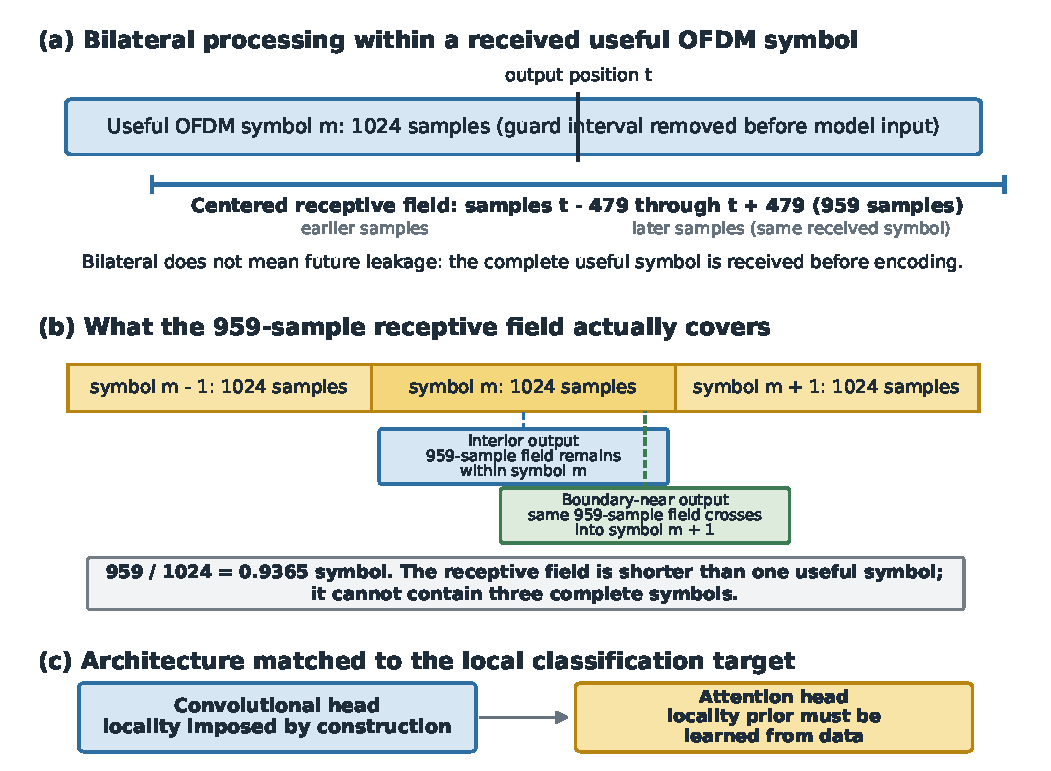
\includegraphics[width=5.5in]{Fig/fig_ofdm_adapt.pdf}
\caption{Architectural adaptations required by OFDM waveform structure.
(a)~Each time-domain sample superposes all $N$ subcarriers, and the cyclic
prefix copies the final $L$ samples to the front, so that sample $k$ equals
sample $k+N$ for $k<L$---a dependence pointing forward in sample index. A causal
kernel masks precisely the side of each position that carries this correlated
content. (b)~The final-layer receptive field spans 959 of 1024 samples;
because it is centered on its output position, it covers most of the current
symbol and generally extends into the neighboring frame. (c)~Occupancy in
frame $m$ depends on the content of frame $m$ alone, so the evidence is local in
time and stationary across frames.}
\label{fig_ofdm_adapt}
\end{figure*}

%----------------------------------------------------------------------------------SUBSUBSECTION IV-D-1
\subsubsection{\textbf{Non-causal kernels within received frames}}
Sequence models for language and for most time series use causal convolution or
masked attention, on the principle that a prediction at time $t$ must not see
$t+1$. Applied inside an OFDM symbol, this principle is not merely unnecessary
but actively harmful. An OFDM symbol is generated by an $N$-point inverse FFT,
so every time-domain sample is a superposition of all $N$ subcarriers:
modulation content is delocalized across the symbol rather than accumulating
from left to right. The cyclic prefix then copies the final $L$ samples of the
IFFT output to the front of the frame, making sample $k$ identical to sample
$k+N$ for $k < L$---a deterministic dependence that points \emph{forward} in
sample index. A causal kernel imposes a temporal ordering the symbol does not
possess and cannot exploit either structure, since the correlations it needs lie
on the side of each position that the mask removes. Centered kernels match the
structure and are used throughout the encoder.

The distinction that matters, and that must be stated carefully in any work of
this kind, is between kernel centering and information leakage. Non-causality
here refers only to the arrangement of the kernel \emph{within frames that have
already been received}. At inference the encoder's input consists exclusively of
past samples; where a centered kernel extends past the leading edge of the
available history, it is zero-padded, never filled with subsequent samples. No
future sample is available to, or used by, the encoder at any point. Kernel
centering within history is a modeling choice; access to the future would be a
methodological error.

%----------------------------------------------------------------------------------SUBSUBSECTION IV-D-2
\subsubsection{\textbf{Receptive field matched to the symbol}}
\label{sec:receptive}
The encoder's stack of dilated convolutions must have a receptive field
comparable to the symbol length if it is to see coherent modulation structure.
% VERIFY: the 959-sample figure below and the 3,559 / 45,761 figures that follow
% were reported separately in the source material and are not consistent with one
% another. Reconcile before submission.
In the configuration studied here, the final layer's receptive field spans 959
samples against a frame length of 1024, so each output position is informed by a
window covering 94\% of a symbol duration. Because the window is centered on its
output position, it is contained within a single frame only for positions lying
near the frame center; for the majority of positions it covers most of the
current symbol together with a portion of the adjacent one. This is not a
defect: occupancy is piecewise constant over the horizons considered, so
context drawn from a neighboring frame is either redundant or, at an occupancy
transition, informative. What the design guarantees is a symbol's worth of
context at every position, not alignment of that context with frame boundaries.
Every output position is therefore informed by at least three full symbols.
Section~VII-B reports the consequence: within the range
tested, the specific kernel sizes matter far less than one would expect, because
once the cumulative receptive field reaches symbol scale, the particular
arrangement of dilations and widths that produced it is secondary.

%----------------------------------------------------------------------------------SUBSUBSECTION IV-D-3
\subsubsection{\textbf{Architecture matched to the classification target}}
\label{sec:ablation_head}
The final stage of the architecture maps a generated time-domain waveform to
frequency-domain occupancy. This is a per-frame problem: whether a sub-block is
occupied in a given frame is determined by the content of that frame alone. The
evidence is therefore local in time and stationary across frames, which is
precisely the inductive bias that a convolutional stack encodes by construction
through weight sharing and restricted support. Attention imposes no such prior;
it can represent the same mapping, but must learn locality and shift covariance
from data, and does so less sample-efficiently at the dataset sizes considered
here. Section~VII-D1 reports the empirical comparison.

%---------------------------------------------------------------------------------------SUBSECTION IV-E
\subsection{\textbf{Framing the Problem as a Queue}}
Finally, the choice of a generative model is justified by the structure
of the process being predicted. New users enter the band according to a
Poisson arrival process, with
\begin{equation}
P(\mathrm{Arrivals} = n) = \frac{e^{-\lambda t}(\lambda t)^n}{n!},
\label{eq:poisson}
\end{equation}
where $t$ is the time in seconds, $\lambda$ is the mean arrival rate, and $n$ the
number of arrivals \cite{Baker}.
Given the history up to the present frame, the number and
timing of arrivals over the next 32 frames is genuinely random. There is
no function of history that returns the correct future; there is only
a distribution over futures.
A generative model represents that
distribution, and the spread of its samples is an honest expression of
what is knowable.
This is the conceptual justification for the entire
architecture and also sets the ceiling on achievable performance:
no predictor can do better than the entropy that the arrival process
permits.

%======================================================================= FIG. 4
\begin{figure*}[!t]
\centering
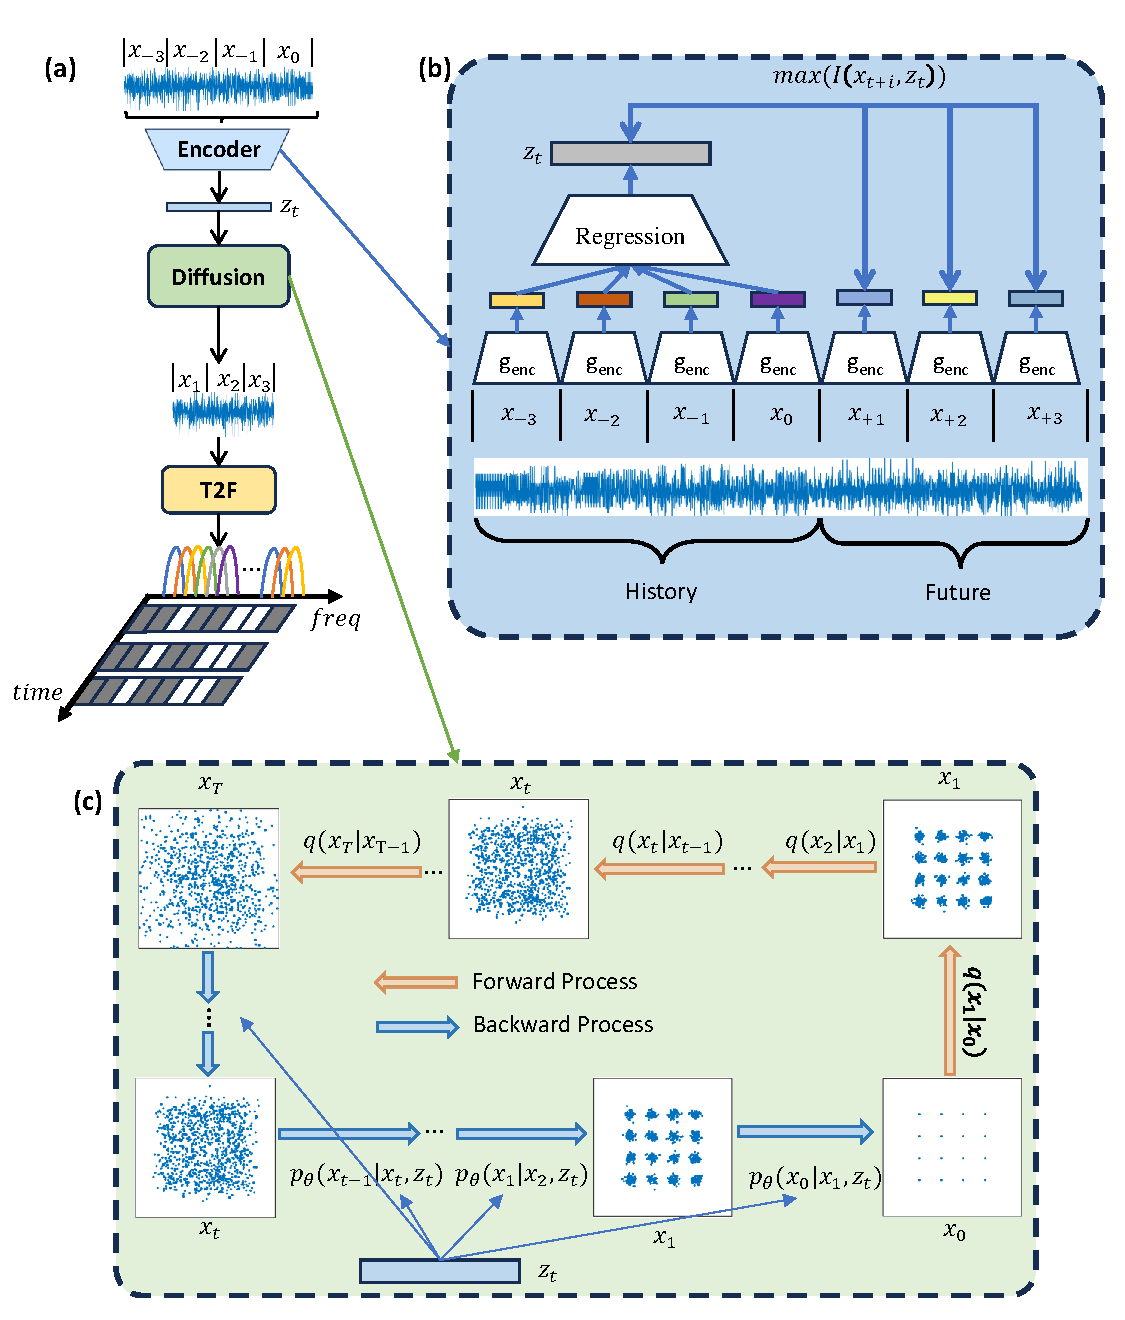
\includegraphics[width=4.5in]{Fig/Slide2.pdf}
% Alternative source file for this figure: Fig/fig_sysdiag
\caption{Reference architecture. (a)~System flow: the history
$[x_{-T_{\mathrm{hst}}},\ldots,x_0]$ is compressed by the latent space
extractor into a context vector $z_t$, which conditions the diffusion
model; the diffusion model generates candidate future waveforms; the T2F
classifier maps each to sub-block occupancy. Four historical 
OFDM-symbol intervals are
drawn for illustration; the deployed configuration uses 128. (b)~Contrastive
training of the encoder, after \cite{Oord2018}. (c)~The
context vector $z_t$ conditions the reverse diffusion process: orange arrows
denote the forward addition of noise from the clean signal $x_0$ to $x_T$, blue
arrows the learned step-by-step denoising back to $x_0$.}
\label{fig_sysdiag}
\end{figure*}
%------------------------------------------------------------------

%=========================================================================================================== SECTION V
\section{\textbf{A Reference Architecture for Sub-Frame Anticipation}}

We now describe a concrete architecture that instantiates the principles
of Section~IV. We present it as a reference design---three composable
stages with defined interfaces---rather than as a fixed proposal, so that
individual stages can be substituted as better components become
available. Figs.~\ref{fig_sysdiag} and \ref{fig:Fig_arch.pipeline} show the
overall flow.

%======================================================================= FIG. 5
\begin{figure*}[!t]
\centering
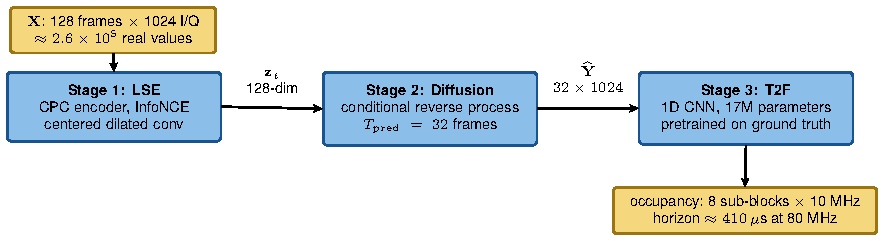
\includegraphics[width=5.5in]{Fig/Fig_arch.pipeline.pdf}
\caption{Stage interfaces and dimensions. The latent space extractor compresses
the observed history to a 128-dimensional context vector $\mathbf{z}_t$; the
conditional diffusion model samples $T_{\mathrm{pred}}=32$ future frames
conditioned on \red{\st{$\mathbf{z}_t$} $z_t$}; the temporal-to-frequency classifier maps each
generated frame to occupancy over eight 10~MHz sub-blocks. Interfaces are
fixed, so individual stages may be substituted.}
\label{fig:Fig_arch.pipeline}
\end{figure*}
%----------------------------------------------------
%---------------------------------------------------------------------------------------SUBSECTION V-A
\subsection{\textbf{Stage 1: Latent Space Extractor}}
The latent space extractor (LSE) is a CPC-trained encoder that maps
$T_{\mathrm{hst}} = 128$ historical OFDM symbol intervals 
to a 128-dimensional context vector. 
Its convolutional backbone uses centered kernels with stride
pattern $[3,3,3,3,3]$ and dilation $[5,5,5,3,3]$, yielding the receptive field
discussed in Section~\ref{sec:receptive}. It is trained with the InfoNCE
objective of (\ref{eq:infonce}), with negatives drawn from a
heterogeneous pool across environments.

The LSE performs two functions that are worth separating. It reduces
$2.6\times10^{5}$ real values to 128, which is what makes the diffusion
stage tractable at all---an advance not available to earlier methods relying on
matched filters or signal power analysis. And, because of the negative-sampling
policy, it is the component responsible for cross-environment generalization: it
is the only stage whose training objective explicitly rewards discarding
environment-specific structure. Section~\ref{sec:zeroshot} examines how much
generalization survives when the diffusion stage---but not the
encoder---faces unseen environments.

%---------------------------------------------------------------------------------------SUBSECTION V-B
\subsection{\textbf{Stage 2: Conditional Diffusion Model}}
The diffusion stage generates plausible future waveforms conditioned on
$z_t$. History is written
$X = \{x_t \in \mathbb{R}^d \mid t = -T_{\mathrm{hst}}, \ldots, 0\}
\in \mathbb{R}^{(T_{\mathrm{hst}}+1)\times d}$
and the prediction target
$Y = \{y_t \in \mathbb{R}^d \mid t = 1, \ldots, T_{\mathrm{pred}}\}
\in \mathbb{R}^{T_{\mathrm{pred}}\times d}$,
where $d$ is the number of samples per frame. The reverse process is
(\ref{eq:reverse}) and training follows (\ref{eq:simple_loss}). The
deployed configuration uses $T_{\mathrm{pred}} = 32$ OFDM symbol intervals, or
 409.6~\us{} when each interval contains a 1024-sample useful symbol at 80~MHz.
This horizon was set by available GPU memory
rather than by any observed degradation in accuracy, a point we return
to in Section~VII-C.

%---------------------------------------------------------------------------------------SUBSECTION V-C
\subsection{\textbf{Stage 3: Temporal-to-Frequency Classifier}}
The temporal-to-frequency (T2F) classifier 
developed in this work maps each generated 1024-sample
OFDM-symbol interval
to the occupancy of eight 10~MHz analysis sub-blocks. It is a 1D
convolutional neural network (CNN) of 17M parameters, 
pretrained on ground-truth
waveforms. In Section VII.D, we demonstrate that using the 
classical CNN for the T2F stage outperforms more modern and advanced 
attention-based models.

Classifying sub-blocks rather than individual subcarriers is a
deliberate simplification that aligns the output with how spectrum is
actually allocated: Wi-Fi and LTE assign groups of subcarriers to a
user, so subcarrier-level labels would carry no additional actionable
information while multiplying the output dimension. The partition is also
portable: each sub-block may serve a single user, or adjacent sub-blocks may be
shared, across a range of wireless standards.

%---------------------------------------------------------------------------------------SUBSECTION V-D
\subsection{\textbf{Fusion With Conventional Sensing}}
The fourth element of the architecture is the one that the case study
showed to be essential, and it is worth stating that it was not part of
the original design. The generated futures and a conventional sensed
estimate of the \emph{current} occupancy are combined by taking the
geometric mean of their per-sub-block confidences. The sensed estimate
may come from an FFT band-power detector or from the T2F classifier
applied to the received history.

The rationale is a division of labor. The sensed estimate is essentially
exact about the present and, because dwell times are long, is therefore a
strong predictor of the near future by simple persistence. The generative
stage is comparatively weak at reproducing the present but carries
information about \emph{impending change}, which persistence by
construction cannot. Fusing them lets each supply what the other lacks.
Section~VII-D quantifies the result.

%---------------------------------------------------------------------------------------SUBSECTION V-E
\subsection{\textbf{End-to-End Fine-Tuning}}
After the stages are trained separately, the encoder and T2F classifier
are fine-tuned jointly with the diffusion parameters frozen, to reduce
the T2F model's sensitivity to the discrepancy between a sampled future
and the realized one. A weighted cross-entropy focuses on gradient
errors:
\begin{align}
L =\; & 0.1 \times \Id\!\left(\hat{S} = S\right) \times
L_{\mathrm{CE}}\!\left(p(\hat{S}), p(S)\right) \nonumber\\
& + 1 \times \Id\!\left(\hat{S} \neq S\right) \times
L_{\mathrm{CE}}\!\left(p(\hat{S}), p(S)\right),
\label{eq:weighted_ce}
\end{align}
where $S$ is the true occupancy, $\hat{S}$ the hard decision obtained by
thresholding the T2F output at 0.5, and $\Id(\cdot)$ the
indicator function. The indicators are non-differentiable and act as
fixed per-element weights, so gradient flows only through the
cross-entropy terms. The asymmetry encourages correction of
diffusion-induced errors without disturbing already-correct predictions.
Table~\ref{tab:params} summarizes the parameter count of each module.

%======================================================================= FIG. 6
\begin{figure*}[!t]
\centering
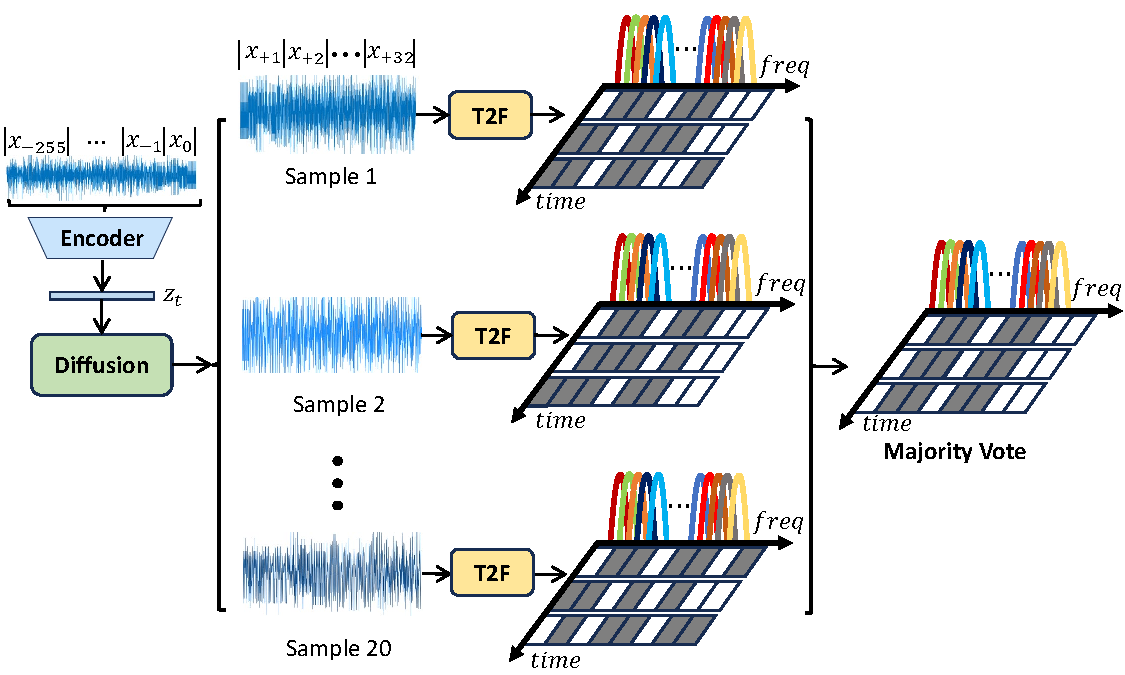
\includegraphics[width=5.5in]{Fig/Slide4.pdf}
\caption{Final inference flow. The encoder (LSE) compresses the historical
signal into a latent space vector $z_t$, which conditions the latent diffusion
model. The diffusion model generates 20 future signals under the same $z_t$. The
CNN-based T2F model processes each generated signal to determine the
frequency-domain occupation of each future time frame, and the per-sub-block
confidences are aggregated across the generated signals to finalize the
prediction.}
\label{fig_inference}
\end{figure*}

%==================================================================== TABLE III
\begin{table}[!t]
\centering
\caption{Model Parameter Summary}
\label{tab:params}
\renewcommand{\arraystretch}{1.2}
\begin{tabular}{@{}lll@{}}
\toprule
\textbf{Module} & \textbf{Parameters} & \textbf{Description} \\
\midrule
Encoder (LSE)   & 0.1B & 1D convolution + Transformer \\
Diffusion model & 0.1B & Transformer with conditioning \\
T2F classifier  & 17M  & 1D convolution \\
\midrule
Total           & 0.2B & --- \\
\bottomrule
\end{tabular}
\end{table}

%============================================================================================================ SECTION VI
\section{\textbf{Evaluating Anticipatory Predictors: A Methodological Note}}

We interrupt the presentation of results to argue a methodological point
that we believe applies to the field generally and not only to the
architecture above. The argument is that the default evaluation practice
in spectrum prediction---compute AUC, accuracy, or F1 (Section III.G) over randomly drawn
evaluation windows---becomes uninformative and can become actively
misleading as prediction horizons shorten toward the frame scale. We set
out the reasoning, the corrections we adopt, and their cost in reported
performance.

%---------------------------------------------------------------------------------------SUBSECTION VI-A
\subsection{\textbf{Dwell-Time Problem}}
Occupancy dwell times in the corpus of Section~VII fall in the 0.1--1~s
range. The prediction horizon is 410~\us. A randomly drawn window
therefore almost never contains an occupancy change. This is not a
peculiarity of our corpus; it follows from the timescale ladder of
Table~\ref{tab:timescales} and will hold for any sub-frame predictor
operating on realistic traffic.

The consequence is stark. In a seeded re-evaluation (seed 42) of the
trained system over 60 windows per environment ($N = 1800$), \emph{not
one window} contained a transition within its 32-frame future. Over such
a set, a predictor that simply copies the current occupancy forward is
exact by construction. Any metric computed over that set measures
primarily the system's ability to reproduce a constant, and a system
with no predictive skill whatsoever can post a respectable number. The
global AUC of the system re-measured at 0.766 over these windows, and
that figure should be understood as characterizing state
\emph{reproduction}, not anticipation.

%---------------------------------------------------------------------------------------SUBSECTION VI-B
\subsection{\textbf{Transition-Conditioned Evaluation}}
The correction is to evaluate on the windows where the quantity of
interest actually occurs. We restrict comparative evaluation to the 135
validation windows whose 32-frame future contains at least one occupancy
flip, and we require that every baseline be evaluated on the same
windows.

This is a demanding protocol, and it should be. It also requires
explicit reporting of the base rate: the occupied-class base rate of
these windows is 0.690, which is the no-skill floor for average
precision (AP). An AP of 0.90 against a base rate of 0.69 is a modest result,
and reporting AP without the base rate invites it to be read as a strong
one.

%---------------------------------------------------------------------------------------SUBSECTION VI-C
\subsection{\textbf{Baselines That Deserve the Name}}
The baseline against which an anticipatory predictor must be measured is
not a weaker learned model. It is \emph{sensed persistence}: estimate the
current occupancy by conventional means and copy it forward. This is what
a deployed system would do today, it is nearly free, and given long dwell
times it is strong. We evaluate it in three forms: driven by an FFT
band-power detector, driven by the T2F classifier applied to the received
history, and in an oracle form driven by ground-truth history labels
(AUC 0.8323).

We further include a \emph{direct label regression} baseline that removes
the generative stage entirely, predicting the $32 \times 8$ occupancy map
from the same frozen encoder context through a 4.7M-parameter head. This
isolates the contribution of generation from the contribution of the
learned representation---a comparison that generative modeling papers
frequently omit, and without which the generative stage cannot be said to
have earned its cost.

%---------------------------------------------------------------------------------------SUBSECTION VI-D
\subsection{\textbf{Operating Points and the Metric That Matters Operationally}}
AUC and AP summarize a ranking over all thresholds. A secondary user does
not operate at all thresholds; it operates at one, chosen to hold
collision probability with the incumbent below a tolerance. We therefore
also report \emph{vacancy detection at 1\% collision}: the fraction of
genuinely vacant sub-blocks identified when the decision threshold is set
so that 1\% of occupied sub-blocks are declared vacant. This is the
quantity that determines how much spectrum a sharing scheme actually
recovers, and as Section~VII-D shows, configurations that are nearly
indistinguishable in AUC differ by a factor of two on it.

%---------------------------------------------------------------------------------------SUBSECTION VI-E
\subsection{\textbf{Aggregation and Reproducibility}}
\label{sec:aggregation}
Two smaller points. First, a fixed-threshold majority vote over ensemble
samples is degenerate in this setting because nearly every per-sample
confidence exceeds 0.5; ranking-based evaluation must use the
ensemble-mean confidence, of which a threshold-swept vote is a single
operating point. Second, evaluation window draws must be seeded and
reported. An earlier, unseeded draw used in our own preliminary ROC
analysis is not recoverable, and we report all comparative results under
the seeded protocol for this reason. We recommend the practice
generally.

%---------------------------------------------------------------------------------------SUBSECTION VI-F
\subsection{\textbf{Clustered Bootstrap Uncertainty}}
Bootstrap standard errors over windows are approximately 0.01 for both
AUC and AP on the transition-conditioned set. Differences smaller than
this are not differences. We state this explicitly because several of the
comparisons in Section~VII fall at or within that level, and reporting
them as ordered would misrepresent the evidence.

%=========================================================================================================== SECTION VII
\section{\textbf{Case Study: An 802.11ax Realization}}

%---------------------------------------------------------------------------------------SUBSECTION VII-A
\subsection{\textbf{Dataset Construction}}
\label{sec:corpus}
The utilized dataset simulates a dynamically changing indoor environment in which
multiple users share a fixed channel through a single transmitter. 
For the appropriate dataset partitioning, we considered the relationship a
mong simulated environments as shown  
in Fig. \ref{fig:fig_sysdiag}. 
Independent waveform realizations, payload partitions, 
component-specific training sets, validation sets, 
and final evaluation sets. Environments and payload 
sequences assigned to final testing are excluded 
from model training and hyperparameter selection. 
The transition-conditioned set is derived only 
after the final test split is fixed.The
resource is 5~s of transmission over 80~MHz centered at
$f_c = 5.25$~GHz. Packet and resource allocation follow IEEE 802.11ax
(High Efficiency, Wi-Fi 6), whose multi-user OFDMA extension divides the
channel into resource units allocated among users \cite{Spirent}. The
generation pipeline is summarized in Fig.~\ref{fig:fig_sysdiag}.

%======================================================================= FIG. 7
\begin{figure*}[!t]
\centering
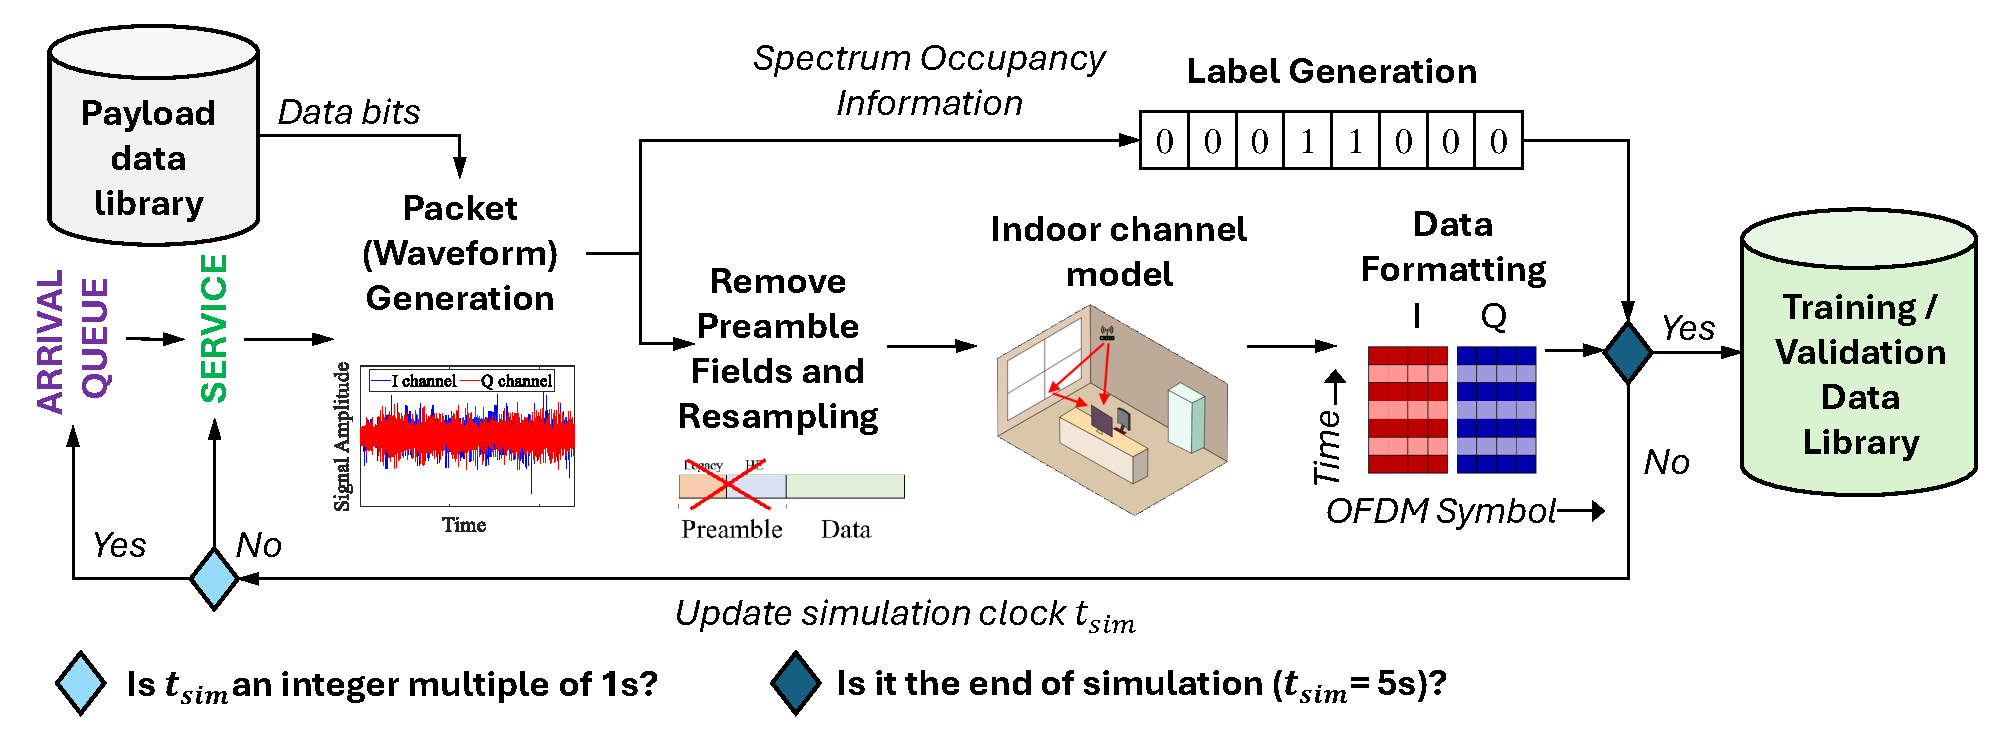
\includegraphics[width=6in]{Fig/fig_sysdiag}
% Alternative source file for this figure: fig_datagen
\caption{Waveform data generation. Users arrive according to a
time-varying Poisson process, are assigned an audio payload and a
modulation and coding scheme, and their packets are generated, passed
through an indoor channel model, and labeled with per-sub-block
occupancy.}
\label{fig:fig_sysdiag}
\end{figure*}

%======================================================================= FIG. 8
\begin{figure*}[!t]
\centering
\includegraphics[width=6in]{Fig/Figure_Data_Part.pdf}
\caption{The dataset partitioning was based on the 
relationship among simulated environments,
independent waveform realizations, payload partitions, 
component-specific training sets, and final evaluation sets. 
Environments and data sequences assigned to the final 
testing were excluded from model training and hyperparameter 
selection.}
\label{fig:Figure_Data_Part}
\end{figure*}

%---------------------------------------------------------------------------------SUBSUBSECTION VII-A-1
\subsubsection{\textbf{User arrivals and payloads}}
Arrivals follow (\ref{eq:poisson}) with a time-varying rate
$\lambda = \lfloor 10 + 10\left|\sin(\pi t / T)\right| \rfloor$ over a
simulation time $T = 5$~s, giving a rise-and-fall load profile
(Fig.~\ref{fig:alloc}a). Each arriving user is assigned an audio payload
drawn from a library of 113 music and speech recordings compiled from
public datasets 
\cite{MUSDB18, Signalogic, WikimediaAudio, VoiceAge, UCLASS, HNM, LibriSpeech}.
Audio was chosen to give realistic diversity of data content, and the binary
representations of these files serve as the transmitted data bits. Raw files
are trimmed to a random length between $10^6$ and $8\times10^6$ samples;
the edited waveform files and their binary representations are available
at \cite{PayloadData}.

%-----------------------------------------------------------------------------------SUBSUBSECTION VII-A-2
\subsubsection{\textbf{Allocation}}
The configuration supports up to 36 users on the 80~MHz channel. To
respect the standard's allocation process, the band is occupied in
multiples of 20~MHz sub-channels, each supporting at most 9 users: below
9 users only 20~MHz is used, and bandwidth is incremented by 20~MHz as
each sub-channel fills. Resource sharing within each 20~MHz sub-channel
is constrained to nine options, corresponding to 802.11ax allocation
indices $\{0, 8, 9, 11, 15, 96, 112, 128, 192\}$
(Fig.~\ref{fig:alloc}b) \cite{MathworksAlloc}. Fig.~\ref{fig:alloc}c
shows the resulting occupation for 9, 15, 19, and 36 users. This
constraint is the origin of the nested-state structure discussed in
Section~\ref{sec:nested}.

%======================================================================= FIG. 9
\begin{figure}[!tp]
\centering
\subfloat[]{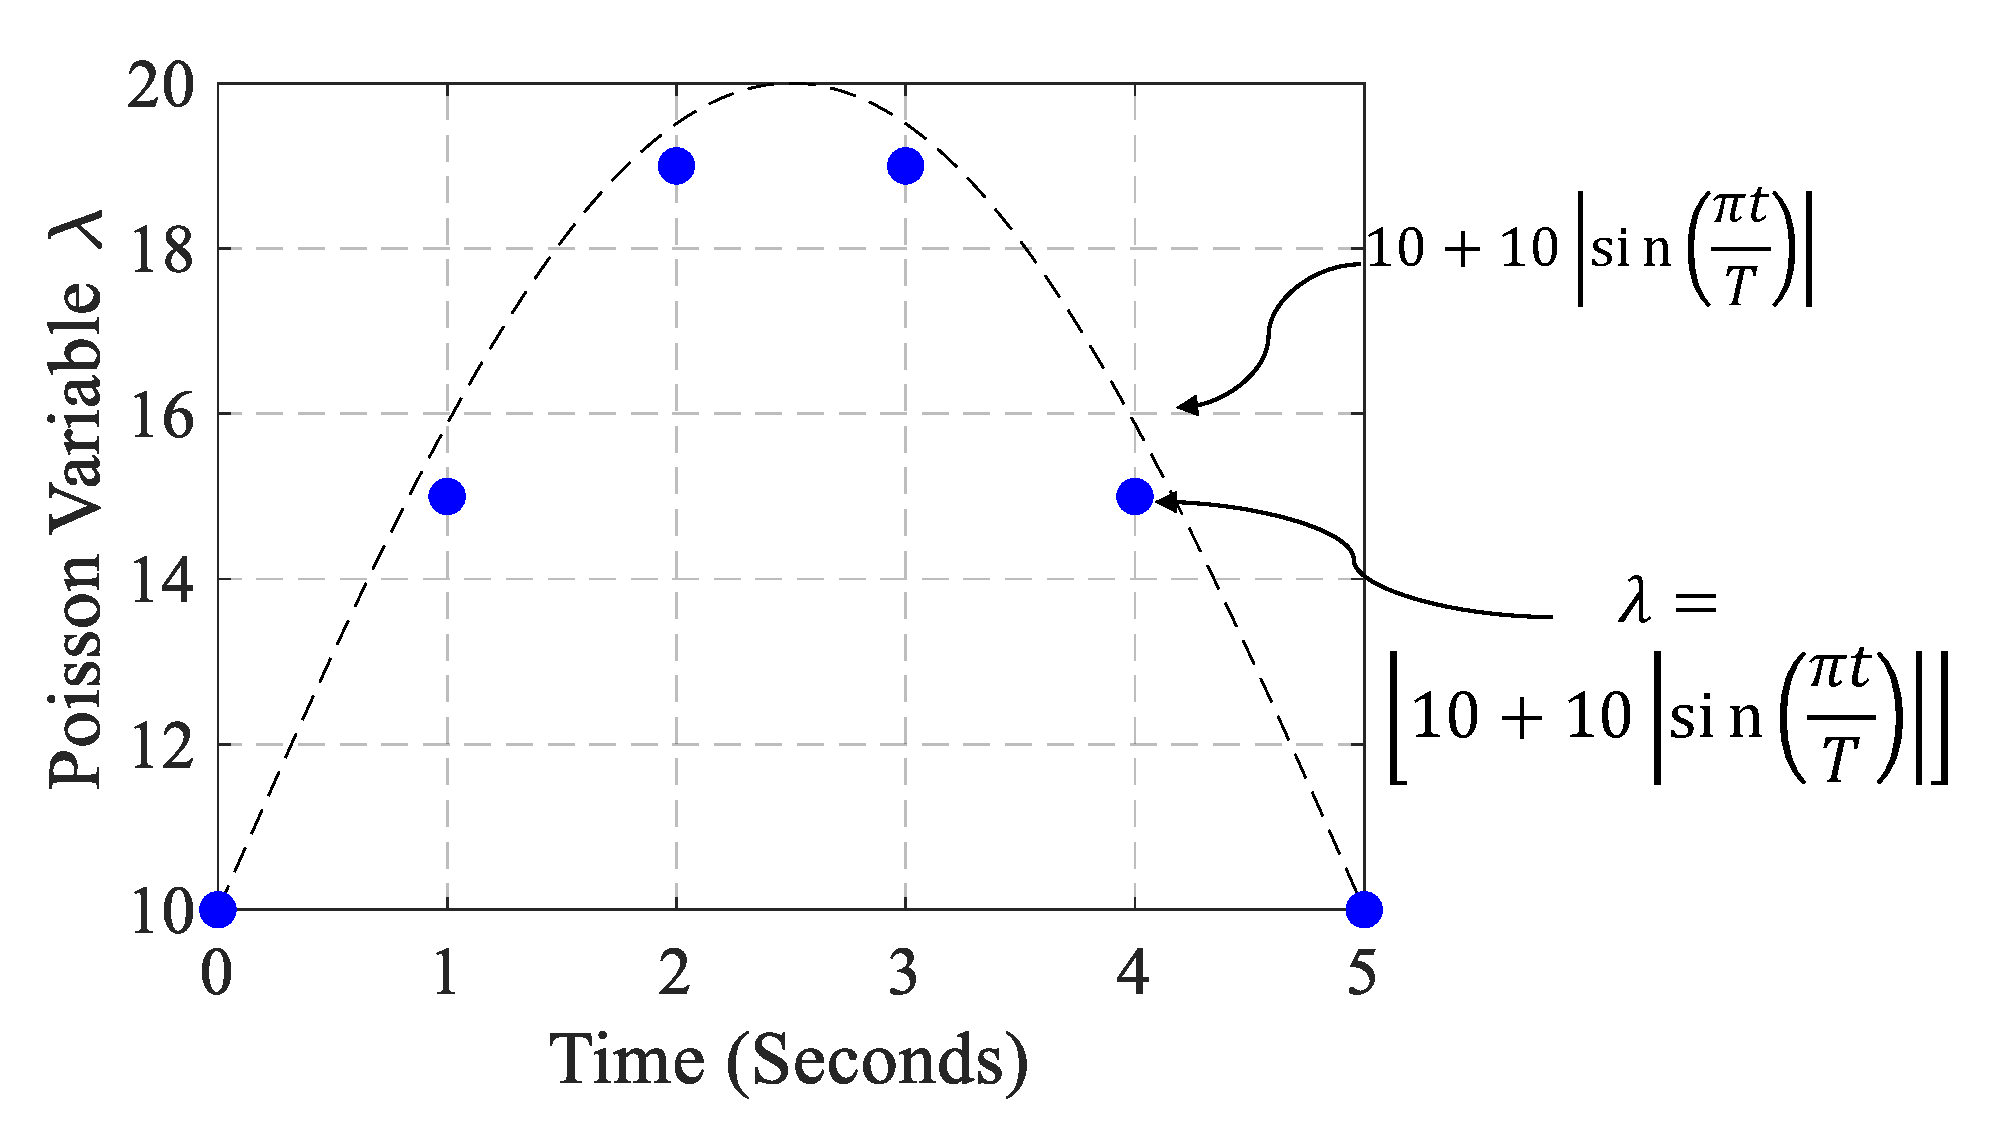
\includegraphics[width=3in]{Fig/Figure S1 - 240930.pdf}%
\label{fig_data2}}
\\[2mm]
\subfloat[]{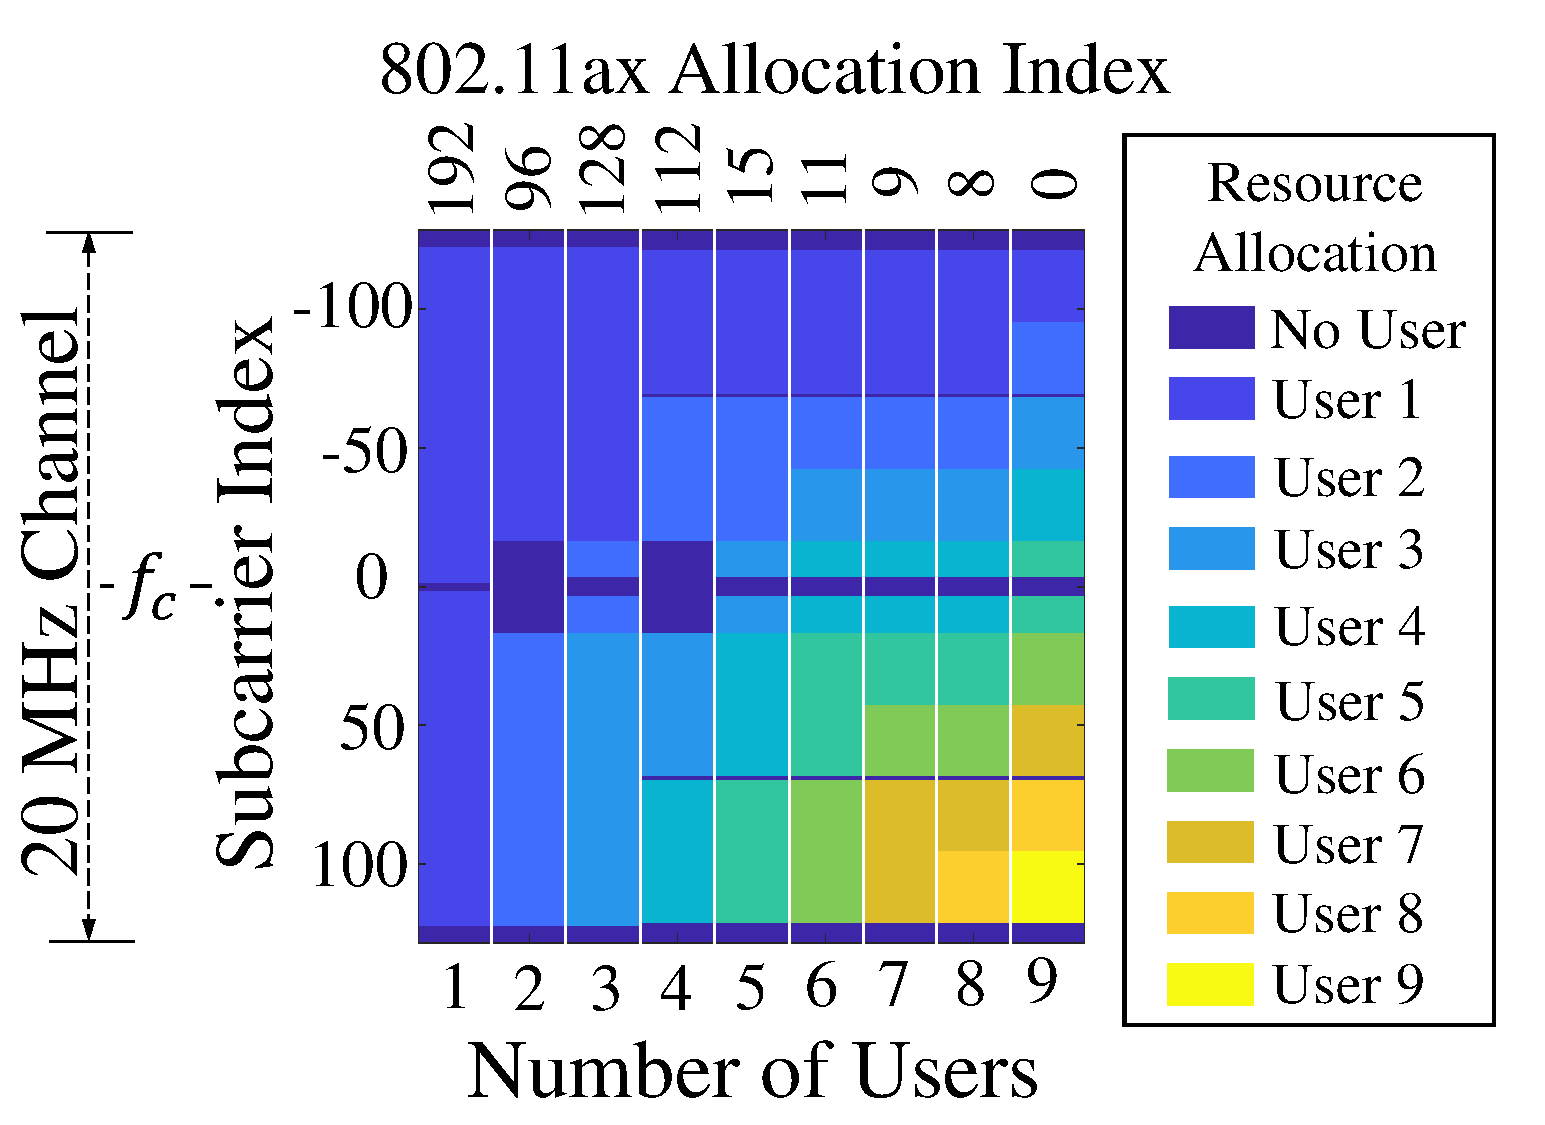
\includegraphics[width=3in]{Fig/Figure S2 - 240930.pdf}%
\label{fig_data3}}
\\[2mm]
\subfloat[]{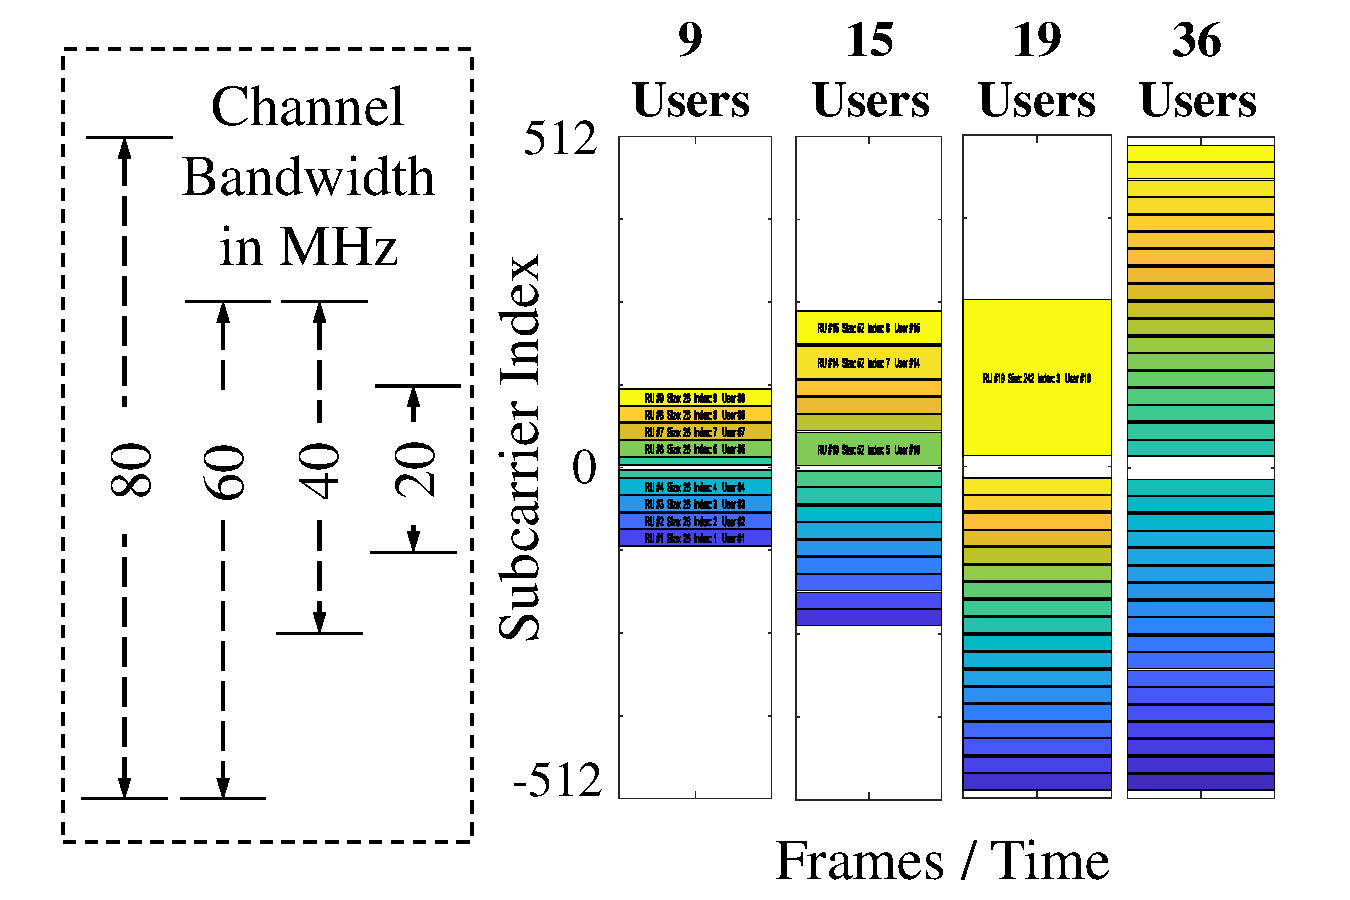
\includegraphics[width=3in]{Fig/Figure S3 - 240930.pdf}%
\label{fig_data4}}
% Alternative source file for this figure: fig_allocation
\caption{(a) Values assigned to the Poisson variable $\lambda$ as the data
generation simulation progresses with time. (b) Allocation of OFDM
sub-carriers and corresponding allocation index per 20~MHz sub-channel;
each 20~MHz sub-channel supports a maximum of 9 users.
(c) Allocation of OFDM sub-carriers and corresponding allocation
index for the 80~MHz channel for 9, 15, 19, and 36 users, respectively.
The subcarrier graph is generated using the MATLAB WLAN toolbox.}
\label{fig:alloc}
\end{figure}

%----------------------------------------------------------------------------------SUBSUBSECTION VII-A-3
\subsubsection{\textbf{Channel and impairments}}
Each user is assigned a modulation and coding scheme from
Table~\ref{tab:mcs}. Waveforms are generated with the MATLAB WLAN
toolbox with APEP (aggregate MAC protocol data unit pre-EOF padding) length set
randomly to 1000 or 1500. Packets stream
continuously for 5~s with new users appearing each second; users are
allocated resources if available, transmit, and exit on completion. All
waveforms are IQ baseband sampled at 80~MHz, passed through an indoor
channel model with additive white Gaussian noise yielding 20--25~dB SNR.
For each 5-s simulation the channel is drawn from the Wi-Fi standard
models A--F \cite{Liu2014}, with 0--2 walls modeled for pathloss and
1--2 walls for pathloss with shadowing, transmitter--receiver separation
of 2--5~m, LDPC coding, and a single space--time stream. These parameter
combinations yield 30 distinct simulated environments spanning a
representative range of indoor propagation conditions; the set is not
exhaustive of real-world environments, but it provides a controlled basis for
validating the framework.

%==================================================================== TABLE IV
\begin{table}[!t]
\centering
\caption{Available Modulation and Coding Schemes}
\label{tab:mcs}
\renewcommand{\arraystretch}{1.15}
\begin{tabular}{@{}cl@{}}
\toprule
\textbf{MCS} & \textbf{Modulation and coding} \\
\midrule
2 & QPSK, rate 1/2 \\
3 & 16-QAM, rate 1/2 \\
4 & 16-QAM, rate 3/4 \\
5 & 64-QAM, rate 2/3 \\
6 & 64-QAM, rate 3/4 \\
7 & 64-QAM, rate 5/6 \\
8 & 256-QAM, rate 3/4 \\
\bottomrule
\end{tabular}
\end{table}

%-----------------------------------------------------------------------------------SUBSUBSECTION VII-A-4
\subsubsection{\textbf{Formatting and labels}}
An ideal receiver removes packet headers and arranges the time-domain
payload so that each OFDM symbol occupies one matrix row, with I and Q
components separated. One 5-s simulation yields a matrix of
$303\,459 \times 1024$. Each row is labeled with eight binary fields, one
per 10~MHz sub-block, taking the value 1 when that sub-block is occupied.
Sixty data files are produced, 30 for training and 30 for validation.

%-----------------------------------------------------------------------------------------SUBSECTION VII-B
\subsection{\textbf{Representation Learning}}
Fig.~\ref{fig:validation}a--c reports encoder validation, with negative samples
drawn from a heterogeneous waveform pool that deliberately excludes samples
closely related to the positive sample's immediate environment. Three findings
are relevant to anyone building such a component.

Increasing history from 64 to 1024 frames yields diminishing returns.
Accommodating 1024 frames required a reduced learning rate and stricter
gradient clipping, lengthening and complicating training, and the
resulting improvement did not justify the cost. Similar behavior holds
for latent dimension (Fig.~\ref{fig:validation}b). The deployed
configuration of 128 history frames and a 128-dimensional latent was
chosen on this basis.

Kernel size is nearly irrelevant. Comparing large kernels against
small under identical stride and dilation shows no significant
difference in convergence (Fig.~\ref{fig:validation}c). As anticipated in
Section~\ref{sec:receptive}, both configurations have a final-layer
receptive field well in excess of one 1024-sample frame, so both already
satisfy the only requirement that matters. The practical implication is that
the small configuration should be preferred, as it reaches the
same regime at a fraction of the cost.

%======================================================================= FIG. 10
\begin{figure*}[!t]
\centering
\subfloat[]{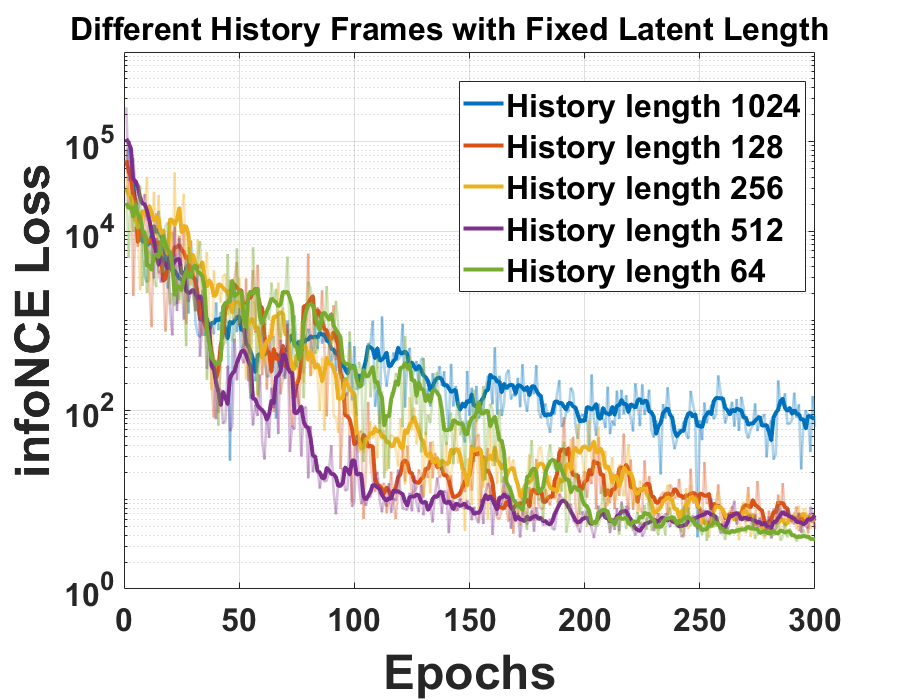
\includegraphics[width=2.2in]{Fig/contrast_test_hist_len.png}%
\label{fig_res1}}
\hfil
\subfloat[]{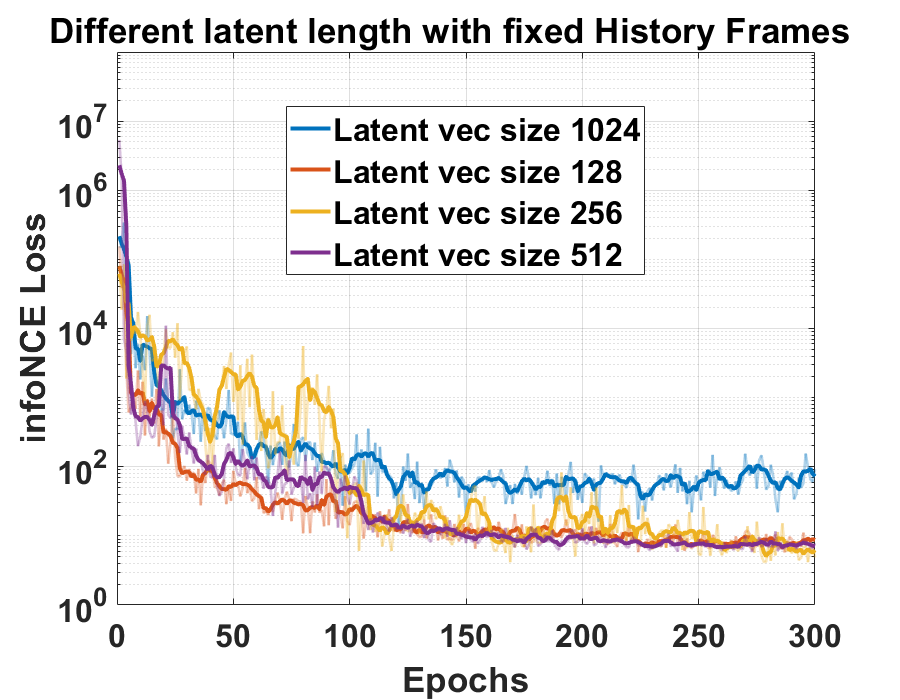
\includegraphics[width=2.2in]{Fig/contrast_test_feature_len.png}%
\label{fig_res2}}
\hfil
\subfloat[]{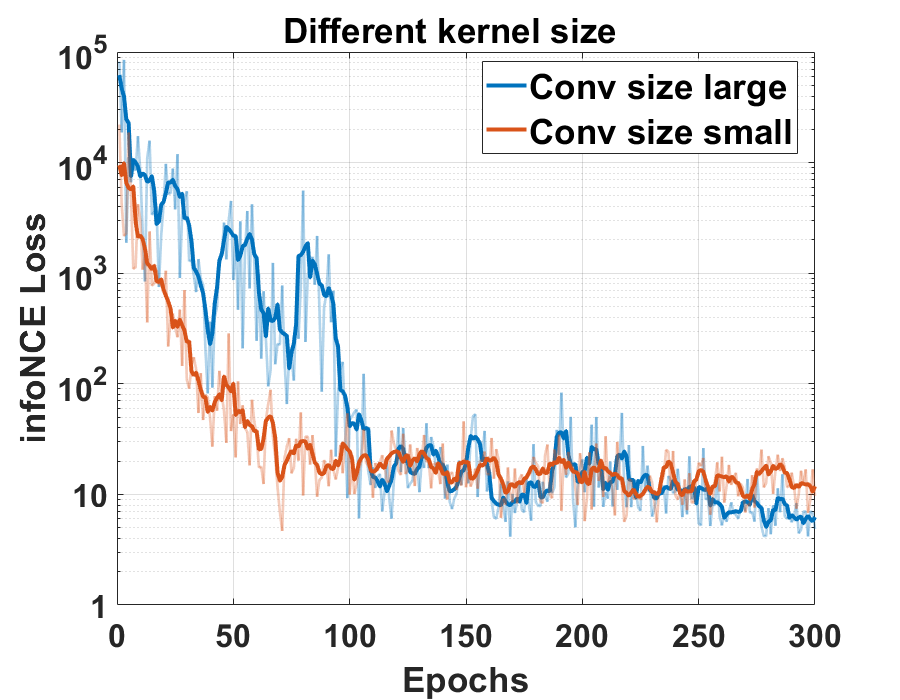
\includegraphics[width=2.2in]{Fig/contrast_test_conv_size.png}%
\label{fig_res3}}
\\[2mm]
\subfloat[]{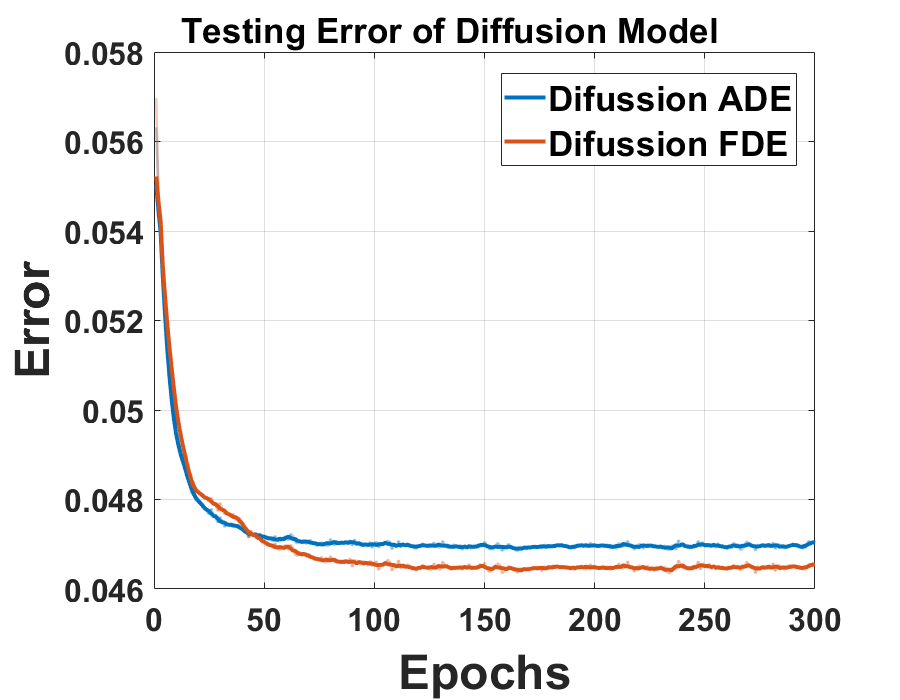
\includegraphics[width=2.2in]{Fig/Testing errors.png}%
\label{fig_res4}}
\hfil
\subfloat[]{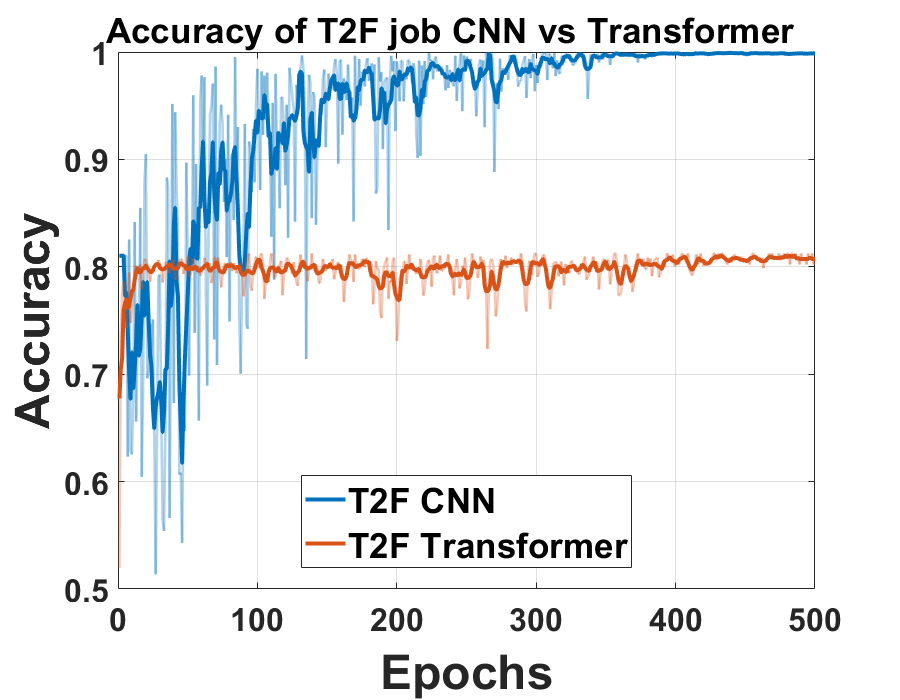
\includegraphics[width=2.2in]{Fig/testing.png}%
\label{fig_res5}}
\hfil
\subfloat[]{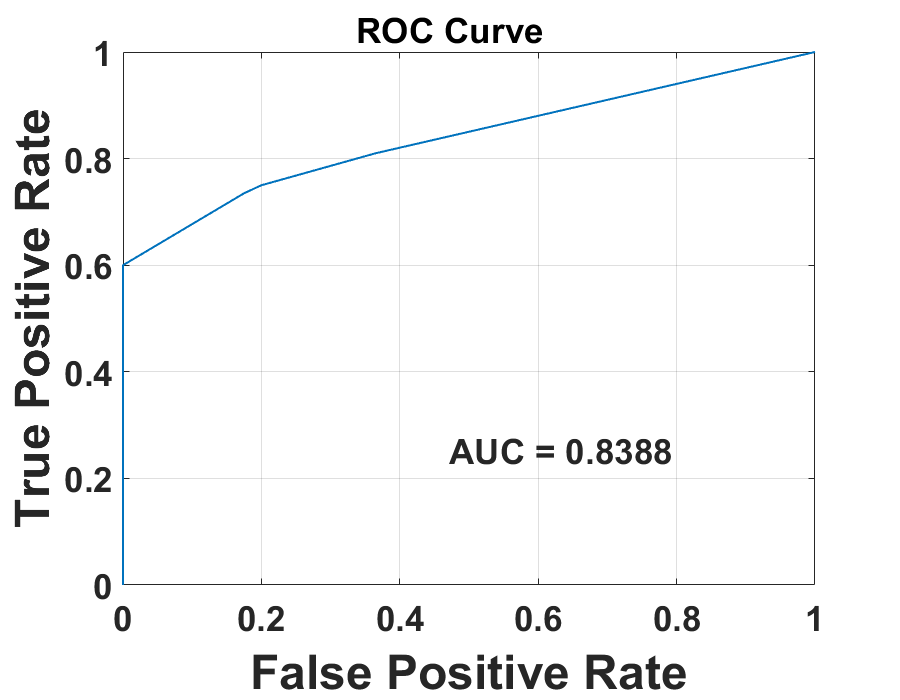
\includegraphics[width=2.2in]{Fig/untitled.png}%
\label{fig_res6}}
% NOTE: source file was named "Testing errors.png"; spaces in graphics filenames
% break \includegraphics. Rename to Testing errors.png (as above) or load grffile.
% Alternative source file for this whole figure: fig_validation
\caption{Validation results. (a) Encoder InfoNCE loss for different
history lengths. (b) Encoder loss for different latent dimensions. (c)
Encoder loss for large ([513, 385, 257, 129, 65]) versus small
([7, 7, 9, 9, 11]) convolution kernels. (d) Diffusion average and final
displacement error. (e) T2F validation accuracy, CNN versus Transformer of
equivalent parameter count. (f) ROC of system-level frequency-block predictions
under the earlier unseeded draw, obtained by sweeping the prediction confidence
threshold; see Section~\ref{sec:aggregation}.}
\label{fig:validation}
\end{figure*}

%---------------------------------------------------------------------------------------SUBSECTION VII-C
\subsection{\textbf{Generative Stage}}
Two measurements characterize the diffusion stage, and both require care
in interpretation.

The first concern is reconstruction error, which for a generative model is
not a performance metric. Because the model samples from a distribution
rather than emitting a point estimate, residual variance against any
single realized waveform is expected. Empirically, a single sampled
future incurs a mean squared error of 0.57 (median across environments),
while the ensemble mean over 20 samples attains 0.35---which matches the
intrinsic variance of the signal itself, 0.34, the irreducible floor
arising from random payload content and channel noise. The gap between
the single-sample and ensemble figures therefore measures the
\emph{diversity} of the sampled futures, not systematic reconstruction
error. It follows that assessment of predictive skill must be conducted
downstream at the occupancy level, which is what Section~\ref{sec:system_results}
does.

The second concern is horizon stability. Average displacement error (ADE)
measures the average error between ground-truth and predicted signals over the
whole horizon, while final displacement error (FDE) measures it at the last
predicted frame; both converge to 0.047
(Fig.~\ref{fig:validation}d). FDE ordinarily exceeds ADE because errors
accumulate over a horizon; their coincidence here indicates that
per-frame error does not grow appreciably across the 32-frame window, so
temporal extrapolation is stable over this span. The 32-frame limit was
imposed by available GPU memory, not by observed degradation, and longer
horizons are an open question, rather than a demonstrated limit.

%---------------------------------------------------------------------------------------SUBSECTION VII-D
\subsection{\textbf{Classifier, System, and Ablations}}

%----------------------------------------------------------------------------------SUBSUBSECTION VII-D-1
\subsubsection{\textbf{Classifier architecture}}
Fig.~\ref{fig:validation}e compares the CNN-based T2F classifier against
a Transformer of equivalent parameter count. The CNN attains near-perfect
validation accuracy after 500 epochs; the Transformer converges to
approximately 0.8. The margin is large and its explanation is
structural, as argued in Section~\ref{sec:ablation_head}: sub-block occupancy in
a frame is determined by that frame's content, which convolution exploits
directly, whereas attention is designed to model inter-frame dependence that is
less informative for this target. The practical reading is that
architecture selection here should follow the locality of the label, not
the prevailing preference for attention; the CNN is additionally the cheaper of
the two to run.

An important corollary follows for error attribution. Because the T2F
classifier is nearly exact on ground-truth waveforms, essentially all
system-level error is attributable to the generative stage---to the gap
between sampled and realized futures. This localizes where further work
should be directed.

%----------------------------------------------------------------------------------SUBSUBSECTION VII-D-2
\subsubsection{\textbf{System-level results}}
\label{sec:system_results}
The inference workflow is shown in Fig.~\ref{fig_inference}: for each input
history, 20 futures are sampled under the same context vector $z_t$, each is
classified by the T2F model, and the per-sub-block confidences are aggregated.
Table~\ref{tab:ablation} reports stage ablations on the 135
transition-containing windows under the protocol of Section~VI; all results use
DDPM sampling except where DDIM is named. Three findings follow.

First, \emph{the generative stage on its own does not surpass sensed
persistence}: 0.8185 AUC against 0.8499 for T2F-driven persistence, with
direct label regression at 0.8382. Pairwise differences among these
single-source configurations sit at or within the bootstrap noise level
of approximately 0.01, so they should be read as comparable rather than
ordered. State-conditioned diffusion, which appends the 8-dimensional
sensed occupancy to the diffusion context, moves the pipeline in the
right direction ($+0.012 \pm 0.010$ AUC).

Second, \emph{fusion is where the value is}. Combining the ensemble
confidence with the sensed estimate attains 0.8844 AUC and 0.9473 AP,
improvements of $+0.034 \pm 0.008$ and $+0.044 \pm 0.007$ over sensed
persistence ($P > 0.999$), approaching the 0.8967 bound of the T2F
classifier applied to the true future waveform. The generated futures
carry information about impending transitions that the sensed current
state does not, and that information is realized only in combination.

Third, \emph{the gain is not specific to diffusion}. A fusion built on
the direct-regression head reaches a statistically indistinguishable
0.8861. The mechanism is the complementarity of any learned predictor
with a sensed prior, not a property unique to the generative
formulation. This is a result we would prefer were otherwise, and it
sets a clear bar for future generative designs: to justify their cost
they must beat a fused regression head, not merely a bare baseline.

%==================================================================== TABLE V
\begin{table*}[!t]
\centering
\caption{Stage Ablations on the 135 Transition-Containing Evaluation Windows}
\label{tab:ablation}
\renewcommand{\arraystretch}{1.2}
\begin{tabular}{@{}lcccc@{}}
\toprule
\textbf{Configuration} & \textbf{Generative stage} & \textbf{AUC} &
\textbf{AP} & \textbf{Vacancy det. @ 1\% collision} \\
\midrule
Sensed persistence (FFT energy detector)      & none    & 0.8156 & 0.9039 & 6.6\% \\
Sensed persistence (T2F on history)           & none    & 0.8499 & 0.9031 & 12.8\% \\
Encoder $\rightarrow$ CNN, direct label regression & removed & 0.8382 & 0.9237 & 5.7\% \\
Proposed (20 samples, ensemble mean)          & full    & 0.8185 & 0.9174 & 6.0\% \\
Proposed, state-conditioned diffusion         & full    & 0.8301 & 0.9233 & 2.9\% \\
\textbf{Proposed $\oplus$ sensed state (fusion)} & full & \textbf{0.8844} & \textbf{0.9473} & 12.8\% \\
T2F on ground-truth waveforms (upper bound)   & oracle  & 0.8967 & 0.9146 & 25.9\% \\
\bottomrule
\end{tabular}
\\[2pt]
\parbox{0.95\textwidth}{\footnotesize Occupied-class base rate 0.690,
which is also the no-skill floor for AP. Bootstrap standard errors over
windows are approximately 0.01 for AUC and AP.}
\end{table*}

%======================================================================= FIG. 11
\begin{figure*}[!t]
\centering
\includegraphics[width=5in]{Fig/Figure_Operation_vacancy.pdf}
\caption{Operational vacancy recovery at 1 \% collision constant. Percentage of genuinely vacant 10 MHz sub-blocks identified by each configuration, conditioned on an evaluation set comprising 135 windows. Diffusion-sensing fusion and T2F-based sensed persistence both recover 12.8 \% of vacant sub-blocks, demonstrating that the fusion model's improvement in ranking metrics does not increase recovered spectrum at the selected operating point. The realized future availability of waveform vacancies is included as an empirical reference.}
\label{fig:Figure_Operation_vacancy.pdf}
\end{figure*}

%----------------------------------------------------------------------------------SUBSUBSECTION VII-D-3
\subsubsection{\textbf{Inference-time ablations}}
Table~\ref{tab:inference} varies the inference-time choices on the same
windows, and the pattern is instructive. Ensemble size barely matters
once fusion is applied: a single sample nearly matches 20. Replacing
DDPM with ten-step DDIM slightly \emph{raises} the fused AUC to 0.8895,
consistent with the observation in Section~\ref{sec:samplers} that DDIM's
deterministic updates collapse the ensemble toward a single effective
sample---which, given the ensemble-size result, costs nothing. Together
these two rows suggest that the sampling diversity the architecture was
designed to exploit is not, in its present form, being exploited; that
is a design weakness worth naming.

The aggregation rule, by contrast, matters a great deal: a
fixed-threshold majority vote reduces the fusion to the sensed estimate
alone, discarding the entire contribution of the generative stage. This
is a failure of calibration rather than of prediction, and it illustrates
why hard-decision aggregation should be avoided in ensembles whose
member confidences are poorly spread.

Finally, at the 1\% collision operating point, sensed persistence and
fusion both identify 12.8\% of vacant sub-blocks against 25.9\% for the
oracle. The AUC gain from fusion does not translate into recovered
spectrum at this operating point---a gap invisible in the ranking
metrics and, we would argue, the single most important number in  
\ref{fig:Figure_Operation_vacancy.pdf} for anyone considering deployment.

%==================================================================== TABLE VI
\begin{table}[!t]
\centering
\caption{Inference-Time Ablations of the Fusion Configuration}
\label{tab:inference}
\renewcommand{\arraystretch}{1.25}
\begin{tabular}{@{}p{1.7cm}p{2.0cm}p{1.9cm}p{1.3cm}@{}}
\toprule
\textbf{Ablation} & \textbf{Setting} & \textbf{AUC} & $\mathbf{\Delta}$ \textbf{AUC} \\
\midrule
Ensemble size & 1 / 5 / 20 samples & 0.8830 / 0.8828 / 0.8844 &
$-0.001$ / $-0.002$ / --- \\
Sampler & DDIM vs.\ DDPM (10 steps each) & 0.8895 & $+0.0051$ \\
Aggregation & majority vote (fixed 0.5) vs.\ mean probability & 0.8499 &
$-0.0345$ \\
\bottomrule
\end{tabular}
\\[2pt]
\parbox{\columnwidth}{\footnotesize $\Delta$ AUC is relative to the
proposed fusion (AUC 0.8844).}
\end{table}

%-------------------------------------------------------------------------FIGURE 12

\begin{figure*}[!t]
\centering
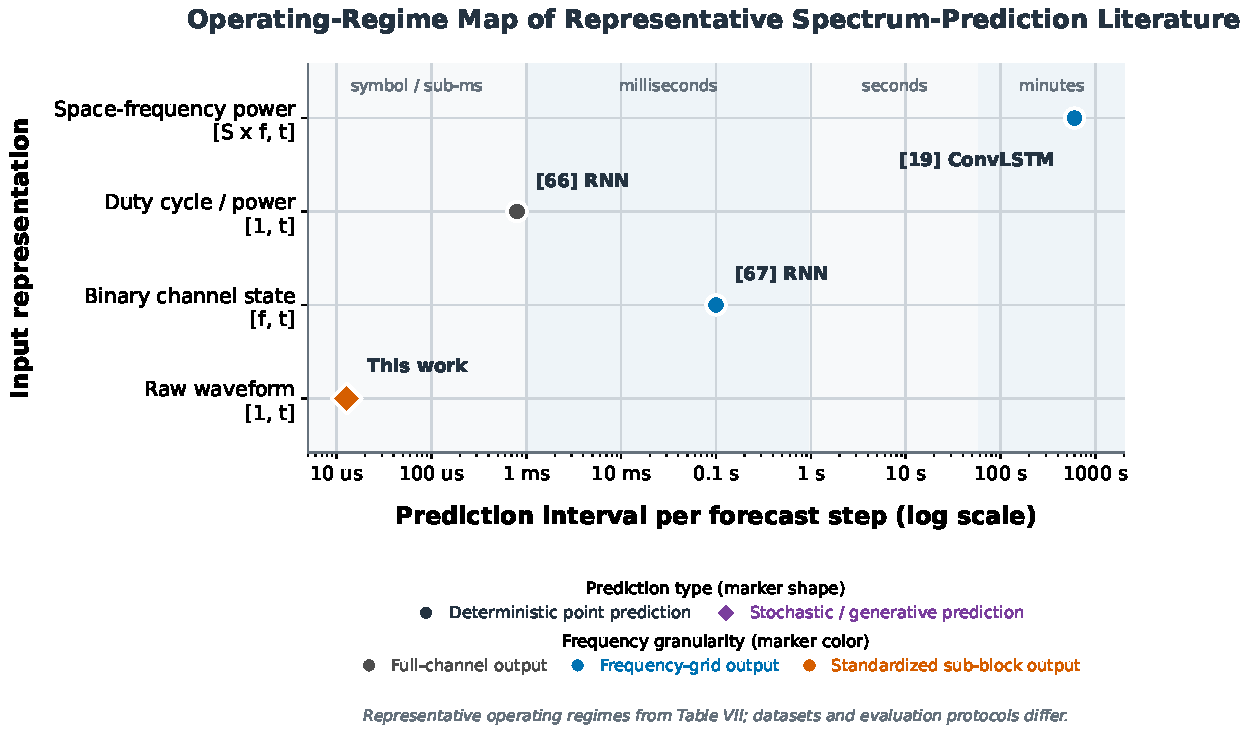
\includegraphics[width=6in]{Fig/Figure_Literature.pdf}
\caption{Operating-regime map of representative spectrum-occupancy 
prediction methods.The horizontal axis shows the prediction interval 
per forecast step on a logarithmic scale, while the vertical axis 
identifies the input representation. Marker shape distinguishes 
deterministic point prediction from stochastic or generative prediction, 
and marker color denotes the frequency granularity of the predicted output. 
The proposed method operates in a distinct regime characterized by 
raw-waveform input, symbol-scale prediction, stochastic generation, 
and standardized sub-block occupancy. The studies are summarized in 
Table VII; their datasets and evaluation protocols differ, so the 
figure compares operating regimes rather than predictive performance.}
\label{fig:Figure_Literature.pdf}
\end{figure*}

%----------------------------------------------------------------------------------SUBSUBSECTION VII-D-4
\subsubsection{\textbf{Qualitative behavior}}
Fig.~\ref{fig:occupancy} illustrates inference where occupancy changes
during the prediction period. The predicted per-sub-block probability at
128~\us\ into the future, aggregated over 20 independent samples,
tracks the ground truth, with disagreement among samples concentrated at
the boundaries of the occupied region---that is, exactly where the
uncertainty genuinely lies. The cumulative view over 12.8--409.6~\us\
shows how confidence evolves with horizon, and confirms that the model
identifies both the end of ongoing transmissions and the onset of new ones
within the prediction window.

%====================================================================== FIG. 10
\begin{figure*}[!tp]
\centering
\subfloat[]{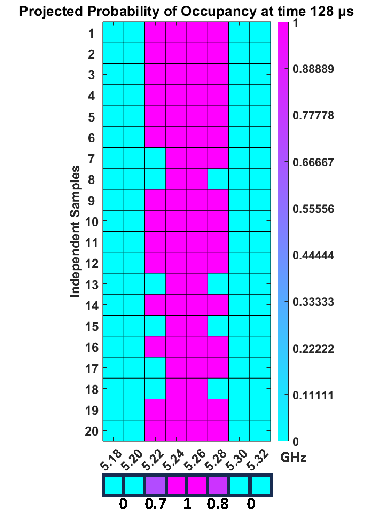
\includegraphics[width=2.3in]{Fig/Slide5a.pdf}%
\label{fig_res7}}
\hfil
\subfloat[]{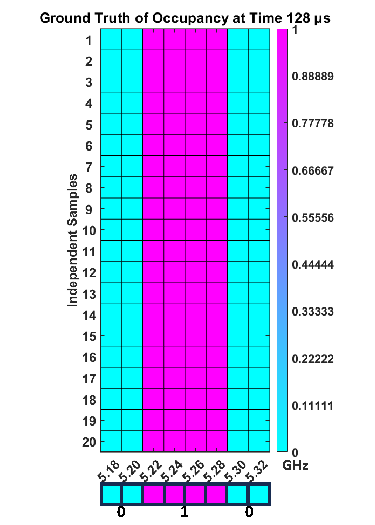
\includegraphics[width=2.3in]{Fig/Slide5b.pdf}%
\label{fig_res8}}
\\[2mm]
\subfloat[]{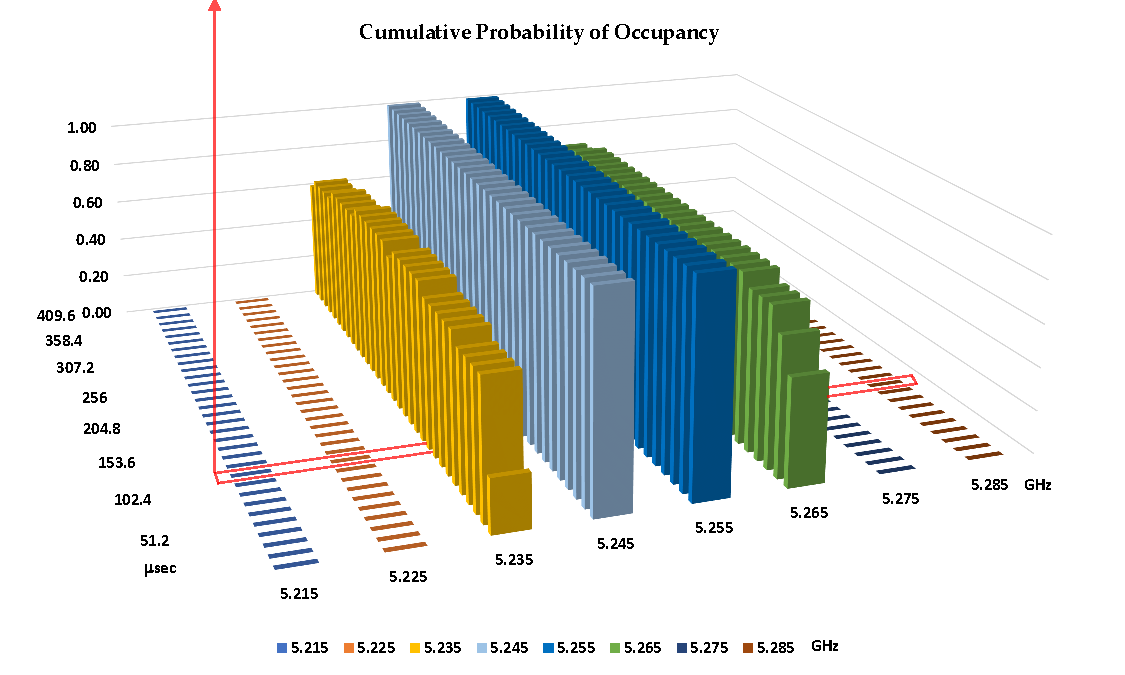
\includegraphics[width=0.85\textwidth]{Fig/Slide5c.pdf}%
\label{fig_res9}}
% Alternative source file for this figure: fig_occupancy
\caption{Future frequency occupation. (a) Predicted occupancy
probability at 128~\us\ ahead from 20 independent diffusion outputs
under the same history. (b) Ground truth at the same instant. (c)
Cumulative occupancy probability across all 20 outputs at each step from
12.8~\us\ to 409.6~\us.}
\label{fig:occupancy}
\end{figure*}

%----------------------------------------------------------------------------------SUBSUBSECTION VII-D-5
\subsubsection{\textbf{Position relative to prior work}}
Table~\ref{tab:comparison} and Fig.\ref{fig:Figure_Literature.pdf} 
places the architecture against representative
prior methods. The comparison is drawn from reported results on different
datasets and is therefore indicative of operating regime rather than a
controlled benchmark---an unavoidable limitation that Section~IX-E
argues the community should remedy. The distinguishing features are the
observable (raw waveform rather than power or labels), the interval
(12.8~\us\ rather than milliseconds to minutes), the frequency granularity
(sub-block rather than full channel), and the presence of explicit dynamic
prediction of arrivals and departures.

%==================================================================== TABLE VII
\begin{table*}[!t]
\centering
\caption{Position Relative to Representative Prior Work$^{1}$}
\label{tab:comparison}
\renewcommand{\arraystretch}{1.25}
\begin{tabular}{@{}llp{2.4cm}p{1.7cm}cccc@{}}
\toprule
\textbf{Work} & \textbf{Method} & \textbf{Input format} &
\textbf{History} & \textbf{Steps} & \textbf{Interval} &
\textbf{Span / blocks} & \textbf{Dynamic} \\
\midrule
\cite{Li2021} & ConvLSTM & Signal power $[S\times f, t]^{2}$ &
Weekly + daily + minutes & $\leq 6$ & 10 min & 790--850 MHz / 60 & \xmark \\
\cite{Umebayashi2023} & RNN & Duty cycle (power) $[1,t]$ &
$\sim$2 ms & 1 & 0.8 ms & 2.436--2.437 GHz / 1 & \xmark \\
\cite{Chirov2023} & RNN & Channel state (0/1) $[f,t]$ &
1 s & 1 & 0.1 s & 390--490 MHz / 5120 & \xmark \\
\textbf{This work} & Generative & \textbf{Raw waveform} $[1,t]$ &
1638.4 \us & \textbf{32} & \textbf{12.8 \us} & 5.21--5.29 GHz / 8 &
\cmark \\
\bottomrule
\end{tabular}
\\[2pt]
\parbox{0.95\textwidth}{\footnotesize $^{1}$Based on results reported in
the respective publications; experimental datasets differ.
$^{2}[S \times f, t]$ denotes a space $\times$ frequency matrix sampled
at successive time points.}
\end{table*}


%----------------------------------------------------------------------------------------SUBSECTION VII-E
\subsection{\textbf{Zero-Shot Transfer to Unseen Environments}}
\label{sec:zeroshot}
The results above draw training and validation from the same 30
environments. To probe generalization we retrain the diffusion model on
environments 1--20 only, holding out 21--30 entirely, with identical
architecture, schedule, and training configuration. The encoder and T2F
classifier are reused unchanged, so the experiment isolates the transfer
behavior of the generative stage.

Evaluation follows the same inference procedure: 20 futures per history
under a common $z_t$, T2F classification of each, majority vote per
sub-block, and threshold sweeping for the ROC. Table~\ref{tab:zeroshot}
gives per-environment AUC. Overall AUC on unseen environments is 0.7589,
against 0.8388 when all 30 environments are included in training, with
F1 of 0.87 at the fixed 0.5 threshold.

The moderate degradation indicates that a substantial fraction of
system-level performance survives when the generative stage operates
outside its training distribution, consistent with the
cross-environment objective of the contrastive representation. Two
caveats bound the claim. The held-out environments are channel
realizations under the same traffic model, not genuinely different
deployment regimes. And joint transfer of all three stages, together
with few-shot adaptation of the encoder and T2F model, remains untested
\cite{Cullen2023,Shaghluf2021,Nasser2021}.


%==================================================================== TABLE VIII
\begin{table}[!t]
\centering
\caption{Zero-Shot System-Level AUC on Held-Out Environments}
\label{tab:zeroshot}
\renewcommand{\arraystretch}{1.15}
\begin{tabular}{@{}cccc@{}}
\toprule
\textbf{Env.} & \textbf{AUC} & \textbf{Env.} & \textbf{AUC} \\
\midrule
21 & 0.7188 & 26 & 0.6762 \\
22 & 0.8244 & 27 & 0.8982 \\
23 & 0.7171 & 28 & 0.7400 \\
24 & 0.7595 & 29 & 0.8048 \\
25 & 0.8179 & 30 & 0.7371 \\
\midrule
\multicolumn{2}{c}{\textbf{Overall}} & \multicolumn{2}{c}{\textbf{0.7589}} \\
\bottomrule
\end{tabular}
\end{table}

%----------------------------------------------------------------------------------------SUBSECTION VII-F
\subsection{\textbf{Over-the-Air Demonstration at Packet Granularity}}
\label{sec:ota}
To establish that the architecture trains and operates on real transmit--receive
chains rather than only on simulated waveforms, we report a packet-granularity
experiment. Here the prediction unit is a Wi-Fi packet rather than an OFDM
frame, so this is a demonstration of architectural viability on measured data,
not a repeat of the frame-level result.

%-----------------------------------------------------------------------------------FIGURE 14 
\begin{figure}[!tbp]
\centering
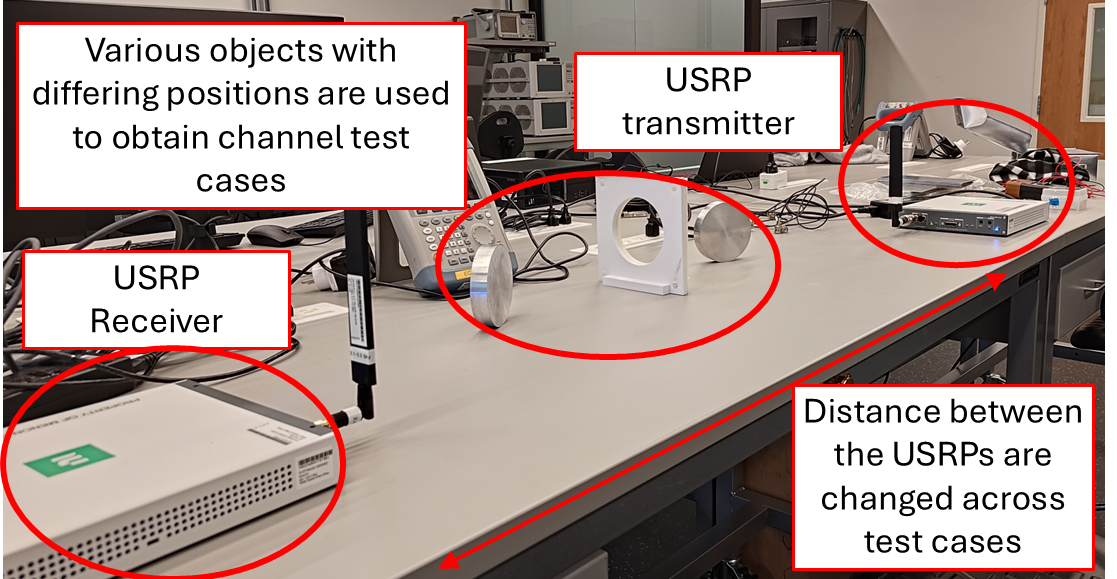
\includegraphics[width=3.4in]{Fig/measurement_setup.png}
% Alternative source file for this figure: fig_usrp
\caption{Wi-Fi transmit--receive link constructed from NI USRP X310
software-defined radios, with objects introduced to vary channel
conditions.}
\label{fig:usrp}
\end{figure}

%---------------------------------------------------------------------------------SUBSUBSECTION VII-F-1
\subsubsection{\textbf{Setup}}
Two National Instruments USRP X310 software-defined radios, each on an
independent computer with 10\,GbE networking, use UBX-160 daughterboards and
5.1--5.9\,GHz blade antennas (Fig.~\ref{fig:usrp}). Radio control, transmission,
and reception are performed in MATLAB 2025a with the appropriate USRP toolboxes;
the receiver uses a modified version of~\cite{MathworksRecover} for over-the-air
packet identification and segmentation.

Three 5-s base scenarios were generated under ideal conditions---without AWGN or
channel impairments---using the method of Section~\ref{sec:corpus}, each
producing about 1200 packets separated by 30\,$\mu$s of idle time, and
transmitted over the air. Packets were sent sequentially in batches of 3--6
owing to computer memory limits. Channel test cases were created by varying
USRP separation (2--4\,ft), placing metallic and dielectric objects and fans
around the radios, and in one case inserting a plywood barrier. The setup sat in
a typical laboratory environment including interference from nearby Wi-Fi
devices and routers. To control dataset quality successful reception 
required an error vector magnitude (EVM)
below $-10$\,dB; for comparison typical packets measured EVM of $-30$\,dB.



%-----------------------------------------------------------------------------------FIGURE 15
\begin{figure}[!tbp]
\centering
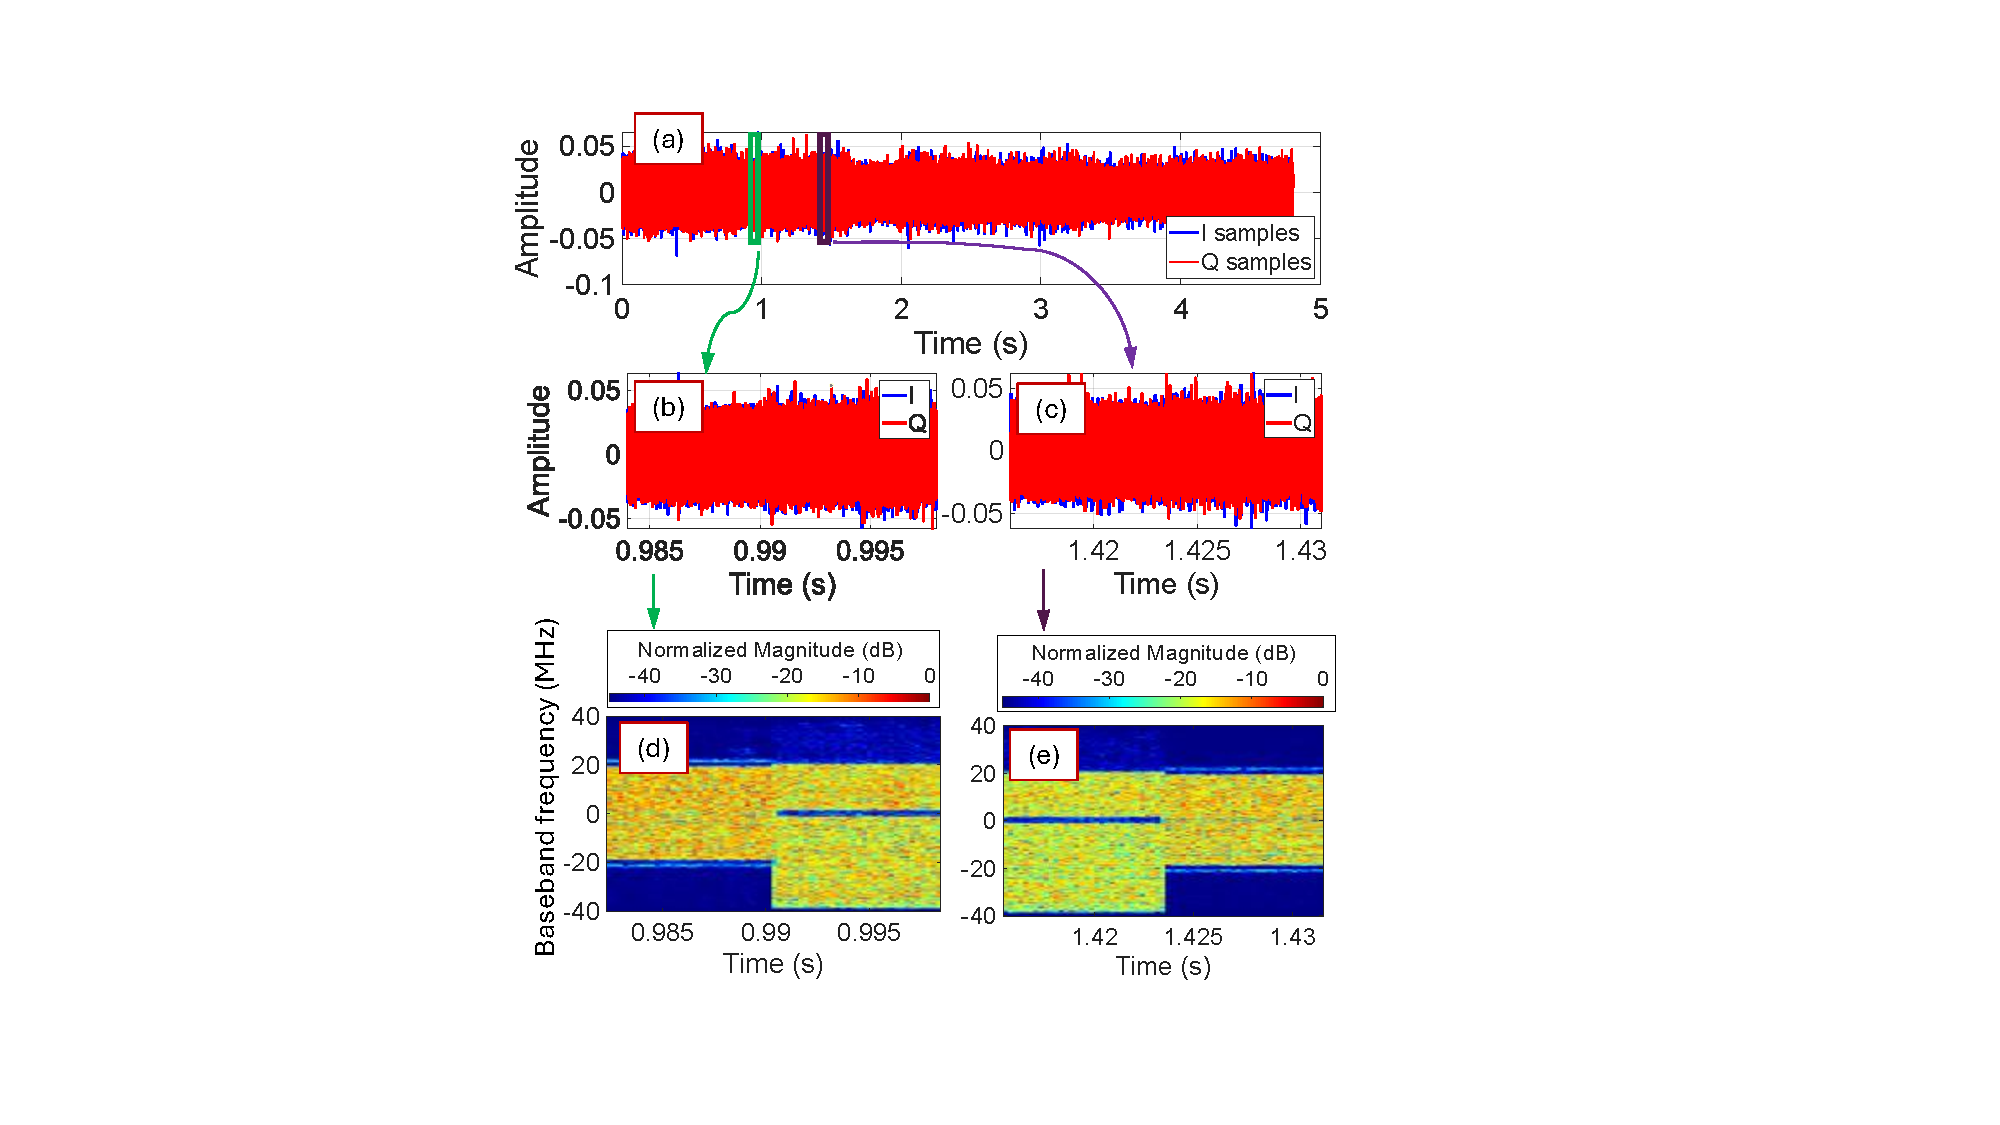
\includegraphics[width=3.4in]{Fig/measurement_data.pdf}
% Alternative source file for this figure: fig_usrp
\caption{A representative measurement using the setup in Fig. \ref{fig:usrp}: (a) Received IQ samples from a full $\approx$ 1200 Wi-Fi packets. Any idle-time between packets is discarded. (b and c) IQ samples from two narrower time slots within the entire reception window. (d) Baseband spectrogram corresponding to IQ samples in (b). (e) Baseband spectrogram corresponding to IQ samples in (c). Packets corresponding to the time windows in (b) and (c) are specifically chosen to show a change in spectrum occupancy. These transitions are rare events and a randomly chosen time window is likely to not have a transition.}
\label{fig:usrp_data}
\end{figure}


%-----------------------------------------------------------------------------------FIGURE 16
\begin{figure}[!tbp]
\centering
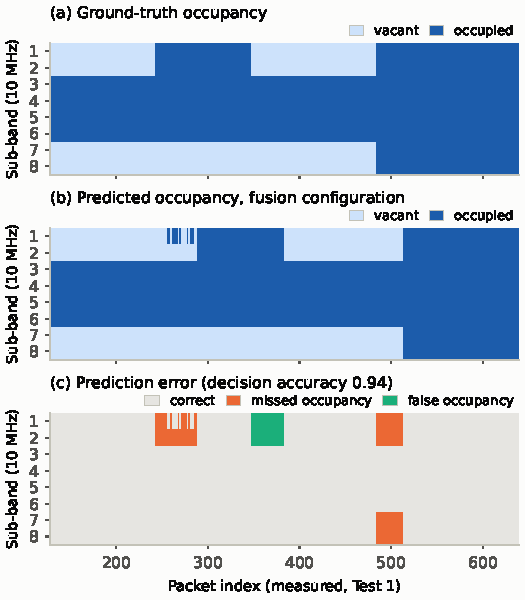
\includegraphics[width=3.4in]{Fig/occupancy_pred_measured.pdf}
\caption{Predicted sub-band occupancy on 512 consecutive received packets (Test~1) for the fusion configuration described in the text: (a) ground truth, (b) prediction, (c) errors. Decision accuracy 0.94.}
\label{fig:occupancy_measured}
\end{figure}


%---------------------------------------------------------------------------------SUBSUBSECTION VII-F-2
\subsubsection{\textbf{Dataset and retraining}}
Each packet is stored as complex baseband I/Q at 80\,MHz and annotated with
ground-truth occupancy of the eight 10\,MHz sub-blocks. Recordings under three
channel conditions, 1202 packets each, serve as three environments. Packets are
resampled to 2048 samples; the system observes 128 consecutive packets and
predicts sub-block occupancy of the following 32.

All three components are retrained with unchanged architectures: the encoder
under the same contrastive objective with in-batch negatives across the three
conditions, the T2F classifier on ground-truth waveforms (where it again attains
near-perfect accuracy), and the diffusion model conditioned on the resulting
$\mathbf{z}_t$. The three are then jointly fine-tuned for six epochs. Inference
mirrors Fig.~\ref{fig_inference}, with one difference from the frame-level
protocol: classifier confidences are averaged over the 20 samples and
thresholded at 0.5, rather than combined by the hard per-sample majority vote of
Section~\ref{sec:system_results}. Given the aggregation result of
Section~\ref{sec:aggregation}---where fixed-threshold voting cost 0.0345
AUC---the ensemble-mean variant is the better-calibrated choice, and we note the
difference so the two sets of numbers are not read as products of an identical
pipeline. Table~\ref{tab:ota} reports the results. For the visualization of Fig.~\ref{fig:occupancy_measured} we apply the fusion configuration of Section~\ref{sec:system_results} to the measured stream, with the sensed estimate taken from the 32 most recent packets rather than the full 128-packet history: at the packet level, occupancy changes only every few hundred packets, and averaging the sensed estimate over the whole history delays the response to each change by tens of packets. The generative pipeline alone reaches a decision accuracy of 0.73 on this stretch, sensing alone 0.93, and their fusion 0.94, with errors confined to the prediction window immediately following each occupancy change.

%==================================================================== TABLE IX
\begin{table}[!t]
\centering
\caption{Model Performance, Over-the-Air Packet-Level Scenario}
\label{tab:ota}
\renewcommand{\arraystretch}{1.2}
\begin{tabular}{@{}lc@{}}
\toprule
\textbf{Metric} & \textbf{Value} \\
\midrule
Sub-block occupancy accuracy (epoch 1) & 0.772 \\
Sub-block occupancy accuracy (best)    & 0.828 \\
F1 score                               & 0.899 \\
Normalized ADE                         & 0.059 \\
Normalized FDE                         & 0.059 \\
\bottomrule
\end{tabular}
\end{table}

%---------------------------------------------------------------------------------SUBSUBSECTION VII-F-3
\subsubsection{\textbf{Scope}}
Two qualifications bound this result and should be read as part of it. The
packet-window sampler draws training and evaluation windows from the same pool,
so these figures characterize in-sample fit on the recorded dataset rather than 
performance on unseen, out-of-sample data; generalization is assessed instead on the simulated
corpus in Section~\ref{sec:zeroshot}. And no ROC analysis is reported for this
dataset. Within that scope, the experiment establishes that the complete
framework---contrastive encoder, conditional diffusion model, and T2F
classifier---trains stably end-to-end on packet-level over-the-air recordings
and reproduces their sub-block occupancy structure at accuracy comparable to the
simulation study.

%========================================================================================================== SECTION VIII
\section{\textbf{Design Principles}}

We abstract five principles from the case study. They are stated as
claims about this class of system rather than about this particular
implementation, and each is accompanied by the evidence that supports it
and the limits of that evidence. A sixth subsection states what the
resulting resolution buys.

%----------------------------------------------------------------------------------------SUBSECTION VIII-A
\subsection{\textbf{Generation Complements Sensing; It Does Not Replace It}}
The strongest finding of the case study is also its most transferable.
Sampled futures alone underperform a sensed persistence baseline
(0.8185 versus 0.8499 AUC), yet fused with it they approach the oracle
bound (0.8844 versus 0.8967). The two sources are informative about
different things: sensing is nearly exact about the present, which
long dwell times make a strong predictor of the near future; generation
is comparatively weak about the present but carries signal about
impending change, which persistence cannot express by construction.

The design implication is that anticipatory predictors should be
architected as \emph{augmentations} of a sensing pipeline, with an
explicit fusion stage, rather than as replacements for one. A system
built to discard the sensed estimate discards most of its own accuracy.

%----------------------------------------------------------------------------------------SUBSECTION VIII-B
\subsection{\textbf{Evaluate Where the Event Occurs}}
When the dwell time exceeds the horizon by three orders of magnitude,
aggregate metrics measure state reproduction, not anticipation. The
same system scores 0.766 AUC over randomly drawn windows---none of which
contained a transition---and 0.884 under fusion on windows that do. The
first number is not a smaller version of the second; it is a
measurement of a different quantity. Transition-conditioned evaluation
with base rates and sensed-persistence baselines reported should be the
default for this class of work.

%----------------------------------------------------------------------------------------SUBSECTION VIII-C
\subsection{\textbf{Match Architecture to the Locality of the Label}}
The CNN classifier reached near-perfect accuracy, whereas a Transformer of
equal size converged to 0.8. The reason is that sub-block occupancy in a
frame is determined by that frame's content; attention's inter-frame
modeling is capacity spent on the wrong dependency. The general
statement is that architecture should follow the locality structure of
the prediction target rather than prevailing practice, and RF signals
have unusually explicit locality structure---symbol boundaries, cyclic
prefixes, resource-unit assignments---that can be read off the standard.

%----------------------------------------------------------------------------------------SUBSECTION VIII-D
\subsection{\textbf{Representation Is the Transfer Bottleneck}}
Zero-shot transfer of the generative stage to ten unseen environments
costs 0.08 AUC, which is moderate given that the diffusion model had
never encountered those channels. That this holds is attributable to the
encoder, whose contrastive objective with cross-environment negatives is
the only part of the system explicitly rewarded for discarding
environment-specific structure. Investment in the representation stage,
and specifically in negative-sampling policy, buys more generalization
per parameter than investment elsewhere.

%----------------------------------------------------------------------------------------SUBSECTION VIII-E
\subsection{\textbf{Inference-Time Choices Can Erase Model-Time Gains}}
Hard-decision majority voting reduced the fused system to the
performance of sensing alone---a loss of 0.035 AUC, larger than the
entire fusion gain, produced by an aggregation rule rather than by any
model deficiency. Meanwhile, the ensemble size the architecture was
designed around proved nearly irrelevant, and a deterministic sampler
that collapses ensemble diversity slightly improved results. These
observations together indicate that the sampling diversity this design
was built to exploit is not presently being exploited, and that
inference-time configuration deserves the same ablation discipline
usually reserved for architecture.

%----------------------------------------------------------------------------------------SUBSECTION VIII-F
\subsection{\textbf{What Sub-Frame Resolution Buys}}
The purpose of all of the above is heterogeneous coexistence. Devices that
today require separate allocations---radar, satellite links, IoT sensors---can
in principle share a band with Wi-Fi if the sub-channel vacancies within an
ongoing transmission can be identified and claimed quickly enough. A secondary
user does not need an entire band to be free, only a few unoccupied
sub-blocks; resolving occupancy to eight 10~MHz sub-blocks within an 80~MHz
band therefore exposes sharing opportunities that full-band methods cannot see,
and anticipating transitions rather than observing them is what allows the
opportunity to be taken before it closes. Whether it can be taken in practice
depends on the latency budget of Section~IX-A, which is not yet met.

%=========================================================================================================== SECTION IX
\section{\textbf{Open Challenges and a Research Agenda}}

The case study establishes feasibility under controlled conditions. It
does not establish deployability, and the distance between the two is the
subject of this section. We treat the obstacles in rough order of how
binding they are.

%---------------------------------------------------------------------------------------SUBSECTION IX-A
\subsection{\textbf{The Latency Budget}}
The most binding constraint is arithmetic. A predictor whose value
derives from 13~\us\ resolution must produce its prediction within a
window comparable to the horizon it predicts---410~\us\ for a 32-frame
forecast---or the prediction expires before it can be acted upon. The
present implementation is roughly 0.2B parameters running a 20-sample
ensemble over a multi-step reverse diffusion process on a
general-purpose GPU. It is not within three orders of magnitude of that
budget.

Five reductions are available and, importantly, they compose:

\begin{enumerate}
\item \emph{Few-step sampling.} The DDIM result of
Table~\ref{tab:inference} shows that ten deterministic steps cost
nothing in accuracy under fusion. Distillation of the sampler to one or
two steps is a well-established direction.
\item \emph{Ensemble reduction.} A single sample nearly matches twenty
once fused, a $20\times$ reduction available immediately.
\item \emph{Incremental encoding.} The 128-frame history advances by one
frame per prediction. Recomputing the entire encoder each step is
wasteful; a streaming encoder amortizes the cost across frames.
\item \emph{Model scale.} An order-of-magnitude parameter reduction, via
distillation \cite{Hinton2015,Cheng2023} or architecture search, is
plausible given that the T2F classifier---the only stage that must be
exact---already achieves near-perfect accuracy at 17M parameters.
\item \emph{Dedicated hardware.} Fixed-function accelerators or
in-memory compute change the constant factor substantially.
\end{enumerate}

A first-order projection combining these places inference latency on the
order of the prediction window. We state plainly that this projection
remains to be demonstrated; no part of it has been implemented on
embedded hardware. We regard it as the single most important item on
this agenda, because every other result in the paper is contingent on
it.

There is also a conceptual escape worth noting. Nothing requires that
the predictor run at the resolution of its output. A predictor that runs
once per millisecond and emits a 410~\us\ forecast is useful if the
forecast remains valid over the interval between invocations---which the
ADE/FDE stability of Section~VII-C weakly supports. Characterizing the
staleness tolerance of these forecasts would relax the budget
considerably and has not been attempted.

%---------------------------------------------------------------------------------------SUBSECTION IX-B
\subsection{\textbf{Impairments, Mobility, and Environment Population}}
The 30 simulated environments are channel realizations of standardized
802.11ax models A--F under a single transmitter, an ideal receiver, and
a common Poisson traffic profile. They exclude carrier frequency and
timing offset, power amplifier nonlinearity, I/Q imbalance, user
mobility, hidden terminals, and co-channel interference from overlapping
basic service sets. Each of these is present in real deployments and each
could degrade the latent representation on which the diffusion model is
conditioned---the more so because the representation is trained
contrastively, and an impairment that is stable within an environment is
exactly the kind of cue a contrastive objective is prone to latch onto.
The claims of this paper should accordingly be read as establishing
feasibility of the architecture under controlled conditions.

The over-the-air experiment of Section~\ref{sec:ota} exercises a genuine
transmit--receive chain, and thereby some of these impairments, but at
packet rather than frame granularity and across three channel conditions
rather than a representative population. The natural next step is a
frame-granularity over-the-air campaign with held-out environments and
deliberate impairment sweeps; this is a substantial measurement
undertaking rather than an incremental extension.

Mobility deserves separate mention. Every result here assumes static or
quasi-static geometry. Under mobility the channel itself becomes
non-stationary within the history window, and it is an open question
whether the contrastive representation degrades gracefully or
catastrophically.

%--------------------------------------------------------------------------------------SUBSECTION IX-C
\subsection{\textbf{Horizon and the Entropy Limit}}
The 32-frame horizon was set by GPU memory, and ADE/FDE stability
suggests headroom. But there is a limit that no amount of memory
removes. Under the Poisson arrival model of (\ref{eq:poisson}), the
entropy of the future occupancy sequence grows with horizon, and beyond
some point no predictor can do better than report the marginal statistics
of the arrival process. Locating that point---deriving an
information-theoretic bound on predictability as a function of horizon
and arrival rate, in the spirit of predictability analyses in other
domains---would tell the field where to stop, which is at least as
useful as another architecture. We are not aware of such an analysis for
sub-frame spectrum occupancy.

%--------------------------------------------------------------------------------------SUBSECTION IX-D
\subsection{\textbf{Standards and Protocol Integration}}
A prediction is only useful if a protocol can act on it. Three
integration questions are open.

\emph{Where does the predictor live?} At the incumbent access point,
which has the allocation information but no incentive to share; at the
secondary device, which must infer everything from the air interface; or
in a coordinating entity analogous to a spectrum access system
\cite{FCC2015CBRS}, which introduces control-plane latency that at
microsecond timescales is prohibitive. The architecture presented here
assumes the second, which is the hardest and the most deployable.

\emph{What does the incumbent guarantee?} Sub-frame sharing places the
secondary user inside the incumbent's transmission opportunity. Existing
coexistence mechanisms---listen-before-talk, energy detection
thresholds, deference rules---were not designed for a secondary user
that transmits concurrently in an adjacent sub-block. Whether such
operation can be made compatible with 802.11 medium access, and what
guard structure in frequency and time it would require, is unresolved.

\emph{How does it generalize across air interfaces?} Nothing in the
architecture is specific to Wi-Fi; the encoder and diffusion stages
consume waveforms and the T2F classifier consumes standard-defined
sub-block structure. Extension to 5G NR, where the resource grid is
richer and the scheduling more centralized, is plausible and untested.
Heterogeneous coexistence---predicting Wi-Fi occupancy from a device
that also serves radar or satellite traffic---is the motivating use case
of this work and remains entirely prospective.

%--------------------------------------------------------------------------------------SUBSECTION IX-E
\subsection{\textbf{Benchmarks and Reproducibility}}
Table~\ref{tab:comparison} compares reported results on different
datasets under different protocols, which is not a comparison. The
field's review literature has noted the absence of common benchmarks
repeatedly \cite{Suriya2022,Wu2017,Tidjani2019,Eltom2018}, and the
problem is worse for sub-frame prediction because the evaluation
subtleties of Section~VI mean that two papers reporting the same metric
on the same data may be measuring different quantities.

What is needed is modest and specific: a public corpus of labeled
waveform captures spanning environments and traffic regimes, with a
fixed split, seeded evaluation windows, mandatory reporting of base
rates and sensed-persistence baselines, and a collision-referenced
operating point. Precedents exist in adjacent problems---labeled
modulation-recognition corpora transformed that subfield
\cite{OShea2018}---and the payload waveforms and binary data used here
are released \cite{PayloadData} as a partial contribution. We would
encourage the community to treat benchmark construction as a
first-class research output.

%--------------------------------------------------------------------------------------SUBSECTION IX-F
\subsection{\textbf{Security and Adversarial Robustness}}
A predictor that grants channel access is an attack surface, and the
literature on adversarial examples in wireless deep learning is already
clear that RF classifiers are vulnerable to small, physically realizable
perturbations \cite{Sadeghi2019}. Two attacks are specific to this
setting. An adversary that transmits a crafted history can induce the
predictor to declare an occupied sub-block vacant, provoking collisions
with a legitimate incumbent---a denial-of-service against the incumbent
executed through the secondary. Conversely, an adversary can induce
persistent false occupancy, denying the secondary the access it is
entitled to. Neither has been studied for waveform-level generative
predictors, and the conditioning bottleneck---a single 128-dimensional
vector through which all history information passes---is an obvious
target. Robustness certification, anomaly detection on the latent, and
fallback to conventional sensing when the two disagree are all
unexplored.

There is a privacy dimension as well. A model that learns to anticipate
transmission boundaries from raw waveforms is, incidentally, a model
that has learned something about traffic patterns. What can be inferred
about a user's activity from a predictor's latent state is a question
that should be asked before such systems are deployed rather than after.

%--------------------------------------------------------------------------------------SUBSECTION IX-G
\subsection{\textbf{Energy}}
Spectrum sharing is justified by efficiency. A scheme that recovers
bandwidth while consuming a GPU's power budget at every secondary node
has not obviously improved anything, and the efficiency accounting should
be done in joules per recovered bit-second-hertz rather than in AUC.
This accounting has not been performed for any waveform-level predictor
we are aware of, including this one, and it may prove to be the binding
constraint on battery-powered secondary devices even if the latency
budget is met.

%--------------------------------------------------------------------------------------SUBSECTION IX-H
\subsection{\textbf{Toward General Radio-Frequency Representation Models}}
Finally, a broader possibility. The encoder in this architecture is
trained on one band, one standard, and one traffic model, and is
discarded when any of those changes. The trajectory of other domains
suggests an alternative: a single self-supervised representation trained
across bands, standards, and environments, with lightweight heads
adapted to specific tasks---occupancy prediction here, but equally
modulation recognition, interference identification, or the sensing side
of integrated sensing and communication \cite{Liu2022ISAC}. The
ingredients are present: contrastive and masked objectives transfer
across domains \cite{Oord2018,Chen2020}, latent-space diffusion makes
high-dimensional generation tractable \cite{Rombach2022}, and raw I/Q is
abundant and requires no annotation. Whether radio signals possess the
shared structure across bands that would make such a model worthwhile is
an empirical question, and we think it is among the more interesting
ones the field could take up.

%============================================================================================================= SECTION X
\section{\textbf{Conclusion}}

Spectrum is managed on the timescale of grants and used on the timescale
of symbols. This paper has argued that the resulting granularity gap is a
principal and addressable source of underutilization, and that closing it
requires three simultaneous departures from established practice:
operating on raw complex baseband waveforms rather than aggregated
observables, predicting at the resolution of individual physical-layer
frames rather than of seconds, and representing user arrival and
departure as a stochastic process from which futures are sampled rather
than as a quantity to be point-estimated.

We surveyed the spectrum prediction literature through the lens of those
three choices, provided tutorial foundations in contrastive
representation learning and denoising diffusion for a wireless
readership, and presented a reference architecture---a contrastive
encoder for cross-environment generalization, a conditional diffusion model
for future waveform generation, and a CNN classifier for sub-block
occupancy---that realizes all three departures. Evaluated on 30 simulated
IEEE 802.11ax channel realizations over a 32-frame horizon, and on the windows
in which sub-channel occupancy actually changes, the architecture attains an AUC
of 0.884 and an average precision of 0.947 when its generated futures
are fused with a sensed estimate of the current state, approaching the
0.897 bound of the classifier given the true future waveform. An
over-the-air experiment on software-defined radios demonstrates that the
full pipeline trains stably on measured packet-level data.

The finding we most wish to carry forward, however, is the one that
qualifies the headline. The generative stage alone does not beat sensed
persistence; a fused direct-regression head performs
indistinguishably from fused diffusion; and at the 1\% collision
operating point that would govern real secondary access, fusion recovers
no more vacant spectrum than sensing alone. Generative modeling in this
setting has demonstrated a real and complementary contribution---
information about impending transitions that the present state does not
contain---but it has not yet demonstrated that its considerable cost is
warranted over simpler learned alternatives. Establishing that, on
shared benchmarks, under a protocol that evaluates where events actually
occur, and within a latency budget that remains three orders of
magnitude away, is the work that follows. State-conditioned generation,
real-world hardware validation, longer-horizon prediction, and extension to
heterogeneous air interface standards are the principal directions we would
identify for that work.

As demand continues to outpace new allocations, the capacity that
remains to be recovered will increasingly be the capacity that is
short-lived and narrow. Systems that can see it will matter. This paper
is an argument that they are buildable, a demonstration of what is
presently achievable, and an accounting of what is not.


\section*{\textbf{Acknowledgment}}
The authors thank the Intelligent Electromagnetic Sensor Laboratories
(iEMSL) at Texas A\&M University for access to facilities and resources
supporting this research; Mr.\ Yi Huang of the University of
Massachusetts, Amherst, for critical comments during the development of
this manuscript; Sanjay Patel and Mariea Sharaf Anzum of Texas A\&M
University for assistance with measurements; and Mohammed Rezaeifar for his 
assistance with a graph/figure.

\begin{thebibliography}{99}
\footnotesize

\bibitem{Azmat2015} F.~Azmat, Y.~Chen, and N.~Stocks, ``Analysis of spectrum occupancy using machine learning algorithms,'' \emph{IEEE Trans. Veh. Technol.}, vol.~65, 2015.

\bibitem{Rahman2021} A.~U. Rahman, M.~A. Kishk, and M.-S. Alouini, ``Improving spectral efficiency of wireless networks through democratic spectrum sharing,'' arXiv:2111.10570, 2021.

\bibitem{Piran2020} M.~J. Piran \emph{et al.}, ``Multimedia communication over cognitive radio networks from QoS/QoE perspective: A comprehensive survey,'' \emph{J. Netw. Comput. Appl.}, vol.~172, 2020, Art.\ no.\ 102759.

\bibitem{Chen2022} M.~Chen, A.~Liu, W.~Liu, K.~Ota, M.~Dong, and N.~N. Xiong, ``RDRL: A recurrent deep reinforcement learning scheme for dynamic spectrum access in reconfigurable wireless networks,'' \emph{IEEE Trans. Netw. Sci. Eng.}, vol.~9, no.~2, pp.~364--376, 2022.

\bibitem{Mitola1999} J.~Mitola and G.~Q. Maguire, ``Cognitive radio: Making software radios more personal,'' \emph{IEEE Pers. Commun.}, vol.~6, no.~4, pp.~13--18, 1999.

\bibitem{Haykin2005} S.~Haykin, ``Cognitive radio: Brain-empowered wireless communications,'' \emph{IEEE J. Sel. Areas Commun.}, vol.~23, no.~2, pp.~201--220, 2005.

\bibitem{FCC2015CBRS} Federal Communications Commission, ``Report and order and second further notice of proposed rulemaking,'' GN Docket No.~12-354, 2015. % VERIFY citation details

\bibitem{NSS2023} National Telecommunications and Information Administration, ``National spectrum strategy,'' U.S. Dept.\ of Commerce, 2023. % VERIFY citation details

\bibitem{Chen2016} Y.~Chen and H.~Oh, ``A survey of measurement-based spectrum occupancy modeling for cognitive radios,'' \emph{IEEE Commun. Surveys Tuts.}, vol.~18, pp.~848--859, 2016.

\bibitem{Wellens2007} M.~Wellens, J.~Wu, and P.~M\"ah\"onen, ``Evaluation of spectrum occupancy in indoor and outdoor scenario in the context of cognitive radio,'' in \emph{Proc. CROWNCOM}, 2007, pp.~420--427.

\bibitem{Engiz2021} B.~Engiz and Y.~Rajab, ``Spectrum occupancy measurements in cellular frequency band in Samsun,'' \emph{Balkan J. Elect. Comput. Eng.}, vol.~9, pp.~138--143, 2021.

\bibitem{Kozlowski2021} S.~Koz{\l}owski and K.~Kurek, ``Channel occupancy measurements in 868 MHz ISM band in residential areas,'' \emph{Sensors}, vol.~21, p.~7805, 2021.

\bibitem{Raouf2023} A.~Raouf, S.~Maeng, I.~Guvenc, \"O.~Ozdemir, and M.~Sichitiu, ``Cellular spectrum occupancy probability in urban and rural scenarios at various UAS altitudes,'' in \emph{Proc. IEEE PIMRC}, 2023, pp.~1--6.

\bibitem{Yucek2009} T.~Yucek and H.~Arslan, ``A survey of spectrum sensing algorithms for cognitive radio applications,'' \emph{IEEE Commun. Surveys Tuts.}, vol.~11, pp.~116--130, 2009.

\bibitem{Muzaffar2024} M.~Muzaffar and R.~Sharqi, ``A review of spectrum sensing in modern cognitive radio networks,'' \emph{Telecommun. Syst.}, vol.~85, pp.~347--363, 2024.

\bibitem{FontSegura2010} J.~Font-Segura and X.~Wang, ``GLRT-based spectrum sensing for cognitive radio with prior information,'' \emph{IEEE Trans. Commun.}, vol.~58, pp.~2137--2146, 2010.

\bibitem{Tian2006} Z.~Tian and G.~Giannakis, ``A wavelet approach to wideband spectrum sensing for cognitive radios,'' in \emph{Proc. CROWNCOM}, 2006, pp.~1--5.

\bibitem{Wellens2010} M.~Wellens and P.~M\"ah\"onen, ``Lessons learned from an extensive spectrum occupancy measurement campaign and a stochastic duty cycle model,'' \emph{Mobile Netw. Appl.}, vol.~15, pp.~461--474, 2010.

\bibitem{Li2021} X.~Li, Z.~Liu, G.~Chen, Y.~Xu, and T.~Song, ``Deep learning for spectrum prediction from spatial--temporal--spectral data,'' \emph{IEEE Commun. Lett.}, vol.~25, no.~4, pp.~1216--1220, 2021.

\bibitem{Ren2021} X.~Ren \emph{et al.}, ``Spatio-temporal spectrum load prediction using convolutional neural network and ResNet,'' \emph{IEEE Trans. Cogn. Commun. Netw.}, vol.~8, no.~2, pp.~502--513, 2021.

\bibitem{Shawel2019} B.~Shawel, D.~Woldegebreal, and S.~Pollin, ``Convolutional LSTM-based long-term spectrum prediction for dynamic spectrum access,'' in \emph{Proc. EUSIPCO}, 2019, pp.~1--5.

\bibitem{He2010} A.~He \emph{et al.}, ``A survey of artificial intelligence for cognitive radios,'' \emph{IEEE Trans. Veh. Technol.}, vol.~59, pp.~1578--1592, 2010.

\bibitem{Xing2013} X.~Xing, T.~Jing, W.~Cheng, Y.~Huo, and X.~Cheng, ``Spectrum prediction in cognitive radio networks,'' \emph{IEEE Wireless Commun.}, vol.~20, pp.~90--96, 2013.

\bibitem{Ding2018} G.~Ding \emph{et al.}, ``Spectrum inference in cognitive radio networks: Algorithms and applications,'' \emph{IEEE Commun. Surveys Tuts.}, vol.~20, pp.~150--182, 2018.

\bibitem{Wang2024} L.~Wang, J.~Hu, C.~Zhang, R.~Jiang, and Z.~Chen, ``Deep learning models for spectrum prediction: A review,'' \emph{IEEE Sensors J.}, vol.~24, pp.~28553--28575, 2024.

\bibitem{Gibson1994} A.~Gibson and L.~Arnett, ``Measurements and statistical modelling of spectrum occupancy,'' in \emph{Proc. Int. Conf. HF Radio Syst. Techn.}, 1994, pp.~150--154.

\bibitem{Percival1997} D.~Percival, M.~Kraetzl, and M.~Britton, ``A Markov model for HF spectral occupancy in central Australia,'' in \emph{Proc. Int. Conf. HF Radio Syst. Techn.}, 1997, pp.~14--18.

\bibitem{Saad2016} A.~Saad, B.~Staehle, and R.~Knorr, ``Spectrum prediction using hidden Markov models for industrial cognitive radio,'' in \emph{Proc. IEEE WiMob}, 2016, pp.~1--7.

\bibitem{Pan2026} G.~Pan, D.~Yau, B.~Zhou, and Q.~Wu, ``Deep learning for spectrum prediction in cognitive radio networks: State-of-the-art, new opportunities, and challenges,'' \emph{IEEE Netw.}, vol.~40, pp.~192--200, 2026.

\bibitem{Chen2011} Z.~Chen, N.~Guo, Z.~Hu, and R.~Qiu, ``Channel state prediction in cognitive radio, Part II: Single-user prediction,'' in \emph{Proc. IEEE Southeastcon}, 2011, pp.~50--54.

\bibitem{Akbar2007} I.~Akbar and W.~Tranter, ``Dynamic spectrum allocation in cognitive radio using hidden Markov models: Poisson distributed case,'' in \emph{Proc. IEEE SoutheastCon}, 2007, pp.~196--201.

\bibitem{Xing2013b} X.~Xing, T.~Jing, Y.~Huo, H.~Li, and X.~Cheng, ``Channel quality prediction based on Bayesian inference in cognitive radio networks,'' in \emph{Proc. IEEE INFOCOM}, 2013, pp.~1465--1473.

\bibitem{Yule1927} G.~Yule, ``On a method of investigating periodicities in disturbed series, with special reference to Wolfer's sunspot numbers,'' \emph{Philos. Trans. Roy. Soc. A}, vol.~226, pp.~267--298, 1927.

\bibitem{Slutsky1937} E.~Slutsky, ``Summation of random causes as the source of cyclic processes,'' \emph{Econometrica}, vol.~5, pp.~105--146, 1937.

\bibitem{Box1978} G.~Box, G.~Jenkins, G.~Reinsel, and G.~Ljung, \emph{Time Series Analysis: Forecasting and Control}. 1978.

\bibitem{Hou2021} Y.~Hou \emph{et al.}, ``Modeling and predictability analysis on channel spectrum status over heavy wireless LAN traffic environment,'' \emph{IEEE Access}, vol.~9, pp.~85795--85812, 2021.

\bibitem{Su2009} J.~Su and W.~Wu, ``Wireless spectrum prediction model based on time series analysis method,'' in \emph{Proc. ACM Workshop Cogn. Radio Netw.}, 2009, pp.~61--66.

\bibitem{Tabassam2011} A.~Tabassam, M.~Suleman, S.~Khan, and S.~Tirmazi, ``Spectrum estimation and spectrum hole opportunities prediction for cognitive radios using higher-order statistics,'' in \emph{Proc. Wireless Advanced}, 2011, pp.~213--217.

\bibitem{Pedraza2016} L.~Pedraza, C.~Suarez, I.~Paez, J.~Trivino, and E.~Rodr\'iguez-Colina, ``Linear algorithms for radioelectric spectrum forecast,'' \emph{Algorithms}, vol.~9, p.~82, 2016.

\bibitem{Tumuluru2010} V.~Tumuluru, P.~Wang, and D.~Niyato, ``A neural network based spectrum prediction scheme for cognitive radio,'' in \emph{Proc. IEEE ICC}, 2010, pp.~1--5.

\bibitem{Yin2011} L.~Yin, S.~Yin, W.~Hong, and S.~Li, ``Spectrum behavior learning in cognitive radio based on artificial neural network,'' in \emph{Proc. IEEE MILCOM}, 2011, pp.~25--30.

\bibitem{Winston2013} O.~Winston, A.~Thomas, and W.~Okello-Odongo, ``Optimizing neural network for TV idle channel prediction in cognitive radio using particle swarm optimization,'' in \emph{Proc. CICSyN}, 2013, pp.~25--29.

\bibitem{Yang2014} L.~Yang, N.~Lv, and Z.~Xu, ``Spectrum prediction for cognitive radio system based on optimally pruned extreme learning machine,'' \emph{Appl. Mech. Mater.}, vol.~536, pp.~430--436, 2014.

\bibitem{Taj2011} M.~Taj and M.~Akil, ``Cognitive radio spectrum evolution prediction using artificial neural networks based multivariate time series modelling,'' in \emph{Proc. European Wireless}, 2011, pp.~1--6.

\bibitem{Yang2013} L.~Yang, X.~Liang, T.~Ma, and K.~Liu, ``Spectrum prediction based on echo state network and its improved form,'' in \emph{Proc. IHMSC}, vol.~1, 2013, pp.~172--176.

\bibitem{Golestanian2014} M.~Golestanian, S.~Iranmanesh, R.~Ghazizadeh, and M.~Azimi, ``A learning automata based spectrum prediction technique for cognitive radio networks,'' \emph{Int. Trans. Elect. Comput. Eng. Syst.}, vol.~2, pp.~93--97, 2014.

\bibitem{Ni2011} S.~Ni and S.~Shen, ``Frequency spectrum access mechanism of cognitive radio based on spectrum prediction,'' in \emph{Proc. IET ICCTA}, 2011, pp.~556--560.

\bibitem{Krizhevsky2012} A.~Krizhevsky, I.~Sutskever, and G.~Hinton, ``ImageNet classification with deep convolutional neural networks,'' in \emph{Adv. Neural Inf. Process. Syst.}, vol.~25, 2012, pp.~1097--1105.

\bibitem{Wang2017} J.~Wang \emph{et al.}, ``Spatiotemporal modeling and prediction in cellular networks: A big data enabled deep learning approach,'' in \emph{Proc. IEEE INFOCOM}, 2017, pp.~1--9.

\bibitem{Ozyegen2020} O.~Ozyegen, S.~Mohammadjafari, E.~Kavurmacioglu, J.~Maidens, and A.~Bener, ``Experimental results on the impact of memory in neural networks for spectrum prediction in land mobile radio bands,'' \emph{IEEE Trans. Cogn. Commun. Netw.}, vol.~6, pp.~771--782, 2020.

\bibitem{Jia2020} M.~Jia, X.~Zhang, J.~Sun, X.~Gu, and Q.~Guo, ``Intelligent resource management for satellite and terrestrial spectrum shared networking toward B5G,'' \emph{IEEE Wireless Commun.}, vol.~27, pp.~54--61, 2020.

\bibitem{Yu2018} L.~Yu, J.~Chen, Y.~Zhang, H.~Zhou, and J.~Sun, ``Deep spectrum prediction in high frequency communication based on temporal-spectral residual network,'' \emph{China Commun.}, vol.~15, pp.~25--34, 2018.

\bibitem{Zhang2021} L.~Zhang and M.~Jia, ``Accurate spectrum prediction based on joint LSTM with CNN toward spectrum sharing,'' in \emph{Proc. IEEE GLOBECOM}, 2021, pp.~1--6.

\bibitem{Ding2020} X.~Ding, L.~Feng, Y.~Zou, and G.~Zhang, ``Deep learning aided spectrum prediction for satellite communication systems,'' \emph{IEEE Trans. Veh. Technol.}, vol.~69, pp.~16314--16319, 2020.

\bibitem{Wen2023} X.~Wen, S.~Fang, Z.~Xu, and H.~Liu, ``Joint multidimensional pattern for spectrum prediction using GNN,'' \emph{Sensors}, vol.~23, 2023.

\bibitem{Li2023} K.~Li \emph{et al.}, ``Boost spectrum prediction with temporal-frequency fusion network via transfer learning,'' \emph{IEEE Trans. Mobile Comput.}, vol.~22, pp.~3209--3223, 2023.

\bibitem{Cheng2023} R.~Cheng, J.~Zhang \emph{et al.}, ``Lightweight spectrum prediction based on knowledge distillation,'' \emph{Radioengineering}, vol.~32, 2023.

\bibitem{Hinton2015} G.~Hinton, O.~Vinyals, and J.~Dean, ``Distilling the knowledge in a neural network,'' arXiv:1503.02531, 2015.

\bibitem{Lin2021} F.~Lin \emph{et al.}, ``Spectrum prediction based on GAN and deep transfer learning: A cross-band data augmentation framework,'' \emph{China Commun.}, vol.~18, pp.~18--32, 2021.

\bibitem{Vaswani2017} A.~Vaswani \emph{et al.}, ``Attention is all you need,'' in \emph{Adv. Neural Inf. Process. Syst.}, vol.~30, 2017.

\bibitem{Pan2023} G.~Pan, Q.~Wu, G.~Ding, W.~Wang, J.~Li, and B.~Zhou, ``An Autoformer-CSA approach for long-term spectrum prediction,'' \emph{IEEE Wireless Commun. Lett.}, vol.~12, pp.~1647--1651, 2023.

\bibitem{Ben2025} C.~Ben \emph{et al.}, ``Enhanced multi-band spectrum prediction using singular spectrum analysis and attention-based BiLSTM,'' \emph{IEEE Trans. Cogn. Commun. Netw.}, vol.~11, pp.~118--126, 2025.

\bibitem{Li2025} S.~Li \emph{et al.}, ``A novel multi-scale time fusion transformer for long-range spectrum occupancy prediction,'' \emph{IEEE Trans. Veh. Technol.}, vol.~74, pp.~9299--9312, 2025.

\bibitem{Guan2025} Z.~Guan, W.~Wen, P.~Wu, C.~Wang, and M.~Xia, ``Hybrid CNN-Transformer based sparse channel prediction for high-mobility OTFS systems,'' \emph{IEEE Wireless Commun. Lett.}, vol.~15, pp.~215--219, 2025.

\bibitem{Xu2024} L.~Xu \emph{et al.}, ``Spectrum prediction for mobile Internet of Things based on a DB-LSTM algorithm,'' \emph{IEEE Trans. Veh. Technol.}, vol.~73, pp.~15395--15406, 2024.

\bibitem{Umebayashi2023} K.~Umebayashi \emph{et al.}, ``Spectrum occupancy prediction based on adaptive recurrent neural networks,'' in \emph{Proc. IEEE WCNC}, 2023.

\bibitem{Chirov2023} D.~S. Chirov and E.~O. Kandaurova, ``Spectrum occupancy prediction algorithm using artificial neural networks,'' in \emph{Proc. Syst. Signals Generating Process.}, 2023, pp.~1--4.

\bibitem{Oord2018} A.~van~den Oord, Y.~Li, and O.~Vinyals, ``Representation learning with contrastive predictive coding,'' arXiv:1807.03748, 2018.

\bibitem{Kingma2014} D.~P. Kingma and M.~Welling, ``Auto-encoding variational Bayes,'' in \emph{Proc. ICLR}, 2014.

\bibitem{Goodfellow2014} I.~Goodfellow \emph{et al.}, ``Generative adversarial nets,'' in \emph{Adv. Neural Inf. Process. Syst.}, vol.~27, 2014.

\bibitem{SohlDickstein2015} J.~Sohl-Dickstein, E.~Weiss, N.~Maheswaranathan, and S.~Ganguli, ``Deep unsupervised learning using nonequilibrium thermodynamics,'' in \emph{Proc. ICML}, 2015.

\bibitem{Ho2020} J.~Ho, A.~Jain, and P.~Abbeel, ``Denoising diffusion probabilistic models,'' in \emph{Adv. Neural Inf. Process. Syst.}, vol.~33, 2020, pp.~6840--6851.

\bibitem{Song2021} Y.~Song \emph{et al.}, ``Score-based generative modeling through stochastic differential equations,'' in \emph{Proc. ICLR}, 2021.

\bibitem{Song2021DDIM} J.~Song, C.~Meng, and S.~Ermon, ``Denoising diffusion implicit models,'' in \emph{Proc. ICLR}, 2021.

\bibitem{Rombach2022} R.~Rombach, A.~Blattmann, D.~Lorenz, P.~Esser, and B.~Ommer, ``High-resolution image synthesis with latent diffusion models,'' in \emph{Proc. IEEE/CVF CVPR}, 2022.

\bibitem{Chen2020} T.~Chen, S.~Kornblith, M.~Norouzi, and G.~Hinton, ``A simple framework for contrastive learning of visual representations,'' in \emph{Proc. ICML}, 2020.

\bibitem{Baker} S.~L. Baker, ``Lecture notes on queuing theory I.'' [Online]. Available: \url{http://web.tecnico.ulisboa.pt/mcasquilho/acad/or/queue/SBakerQueuingI.pdf}

\bibitem{Spirent} ``Key considerations for Wi-Fi 6E testing.'' [Online]. Available: \url{https://www.spirent.com/assets/white-paper-key-considerations-for-wi-fi-6e-testing}

\bibitem{MathworksAlloc} MathWorks, ``Allocation index in HE MU transmission.'' [Online]. Available: \url{https://www.mathworks.com/help/wlan/gs/he-mu-transmission.html}

\bibitem{Liu2014} J.~Liu, R.~Porat, N.~Jindal, V.~Erceg, S.~Azizi \emph{et al.}, ``IEEE 802.11ax channel model document,'' Wireless LANs, IEEE 802.11, 2014.

\bibitem{MUSDB18} ``MUSDB18-HQ: An uncompressed version of MUSDB18.'' [Online]. Available: \url{https://doi.org/10.5281/zenodo.3338373}

\bibitem{Signalogic} ``Speech codec WAV samples.'' [Online]. Available: \url{https://www.signalogic.com/index.pl?page=speech_codec_wav_samples}

\bibitem{WikimediaAudio} ``Wikimedia Commons: Audio files.'' [Online]. Available: \url{https://commons.wikimedia.org/wiki/Category:Audio_files}

\bibitem{VoiceAge} VoiceAge Corporation. [Online]. Available: \url{https://voiceage.com/Audio-Samples-AMR-WB.html}

\bibitem{UCLASS} University College London conversation data. [Online]. Available: \url{https://www.uclass.psychol.ucl.ac.uk/Release2/Conversation/AudioOnly/wav/}

\bibitem{HNM} ``Minimization of transition noise and HNM synthesis in very low bit rate speech coding.'' [Online]. Available: \url{https://doi.org/10.1007/3-540-44805-5_41}

\bibitem{LibriSpeech} ``OpenSLR LibriSpeech ASR corpus.'' [Online]. Available: \url{http://www.openslr.org/12}

\bibitem{PayloadData} ``Audio files in binary format and corresponding .wav file for payload data in communication systems.'' [Online]. Available: \url{https://doi.org/10.18738/T8/B85VC9}

\bibitem{MathworksRecover} MathWorks, ``Recover and analyze packets in 802.11 waveform,'' MATLAB WLAN Toolbox documentation, 2025. [Online]. Available: \url{https://www.mathworks.com/help/wlan/ug/recover-and-analyze-packets-in-802-11-waveform.html}

\bibitem{Cullen2023} A.~Cullen, B.~Rubinstein, K.~Sithamparanathan, B.~Flower, and P.~Leong, ``Predicting dynamic spectrum allocation: A review covering simulation, modelling, and prediction,'' \emph{Artif. Intell. Rev.}, vol.~56, pp.~1--39, 2023.

\bibitem{Shaghluf2021} N.~Shaghluf and T.~A. Gulliver, ``Energy and spectrum efficiency in predictive-cooperative cognitive radio networks,'' \emph{Wireless Netw.}, vol.~27, pp.~5297--5311, 2021.

\bibitem{Nasser2021} A.~Nasser, H.~Al~Haj~Hassan, J.~Abou~Chaaya, A.~Mansour, and K.-C. Yao, ``Spectrum sensing for cognitive radio: Recent advances and future challenge,'' \emph{Sensors}, vol.~21, p.~2408, 2021.

\bibitem{Suriya2022} M.~Suriya, ``Study of spectrum prediction techniques in cognitive radio networks,'' in \emph{Proc. ICACCS}, vol.~1, 2022.

\bibitem{Wu2017} J.~Wu and Y.~Li, ``A survey of spectrum prediction methods in cognitive radio networks,'' \emph{AIP Conf. Proc.}, vol.~1834, no.~1, 2017.

\bibitem{Tidjani2019} S.~Tidjani and Z.~Hammoudi, ``A survey on spectrum prediction methods in cognitive radio networks,'' \emph{Int. J. Comput.}, vol.~8, no.~2, pp.~24--31, 2019.

\bibitem{Eltom2018} H.~Eltom \emph{et al.}, ``Statistical spectrum occupancy prediction for dynamic spectrum access: A classification,'' \emph{EURASIP J. Wireless Commun. Netw.}, vol.~2018, pp.~1--17, 2018.

\bibitem{OShea2018} T.~J. O'Shea, T.~Roy, and T.~C. Clancy, ``Over-the-air deep learning based radio signal classification,'' \emph{IEEE J. Sel. Topics Signal Process.}, vol.~12, no.~1, pp.~168--179, 2018.

\bibitem{Sadeghi2019} M.~Sadeghi and E.~G. Larsson, ``Adversarial attacks on deep-learning based radio signal classification,'' \emph{IEEE Wireless Commun. Lett.}, vol.~8, no.~1, pp.~213--216, 2019.

\bibitem{Liu2022ISAC} F.~Liu \emph{et al.}, ``Integrated sensing and communications: Toward dual-functional wireless networks for 6G and beyond,'' \emph{IEEE J. Sel. Areas Commun.}, vol.~40, no.~6, pp.~1728--1767, 2022.

\end{thebibliography}

\vfill

\end{document}
